% !TEX root = ../main.tex
%

The performance of the analysis to distinguish different CP scenarios in the coupling of the Higgs boson to gluons is 
quantitatively evaluated by a measurement of the CP mixing angle $\alpha$ in a MC simulation.
For this purpose a pseudo-data set is constructed from the background-plus-SM-signal hypothesis for a scalar SM Higgs boson. To perform the measurement a likelihood function is constructed and maximized
for various signal+background scenarios that depend on $\alpha$. The scenario that shows the best compatability of the background-plus-signal hypothesis
 and the pseudo-data set is, thus, equivalent to a measurement of the actual mixing angle realized in (pseudo-)data.


\subsection{Signal model}\label{SA:physicsmodel}
As seen before, a different CP scenario predicts a different shape and  yield of the signal templates. Since the production of dedicated Monte Carlo samples for a larger number of 
CP scenarios consumes a lot of CPU time and is thus very expensive, a model is developed that allows for 
the reweighting of three existing templates to provide shape and yield of any CP scenario as a function of the mixing angle $\alpha$.
In this analysis, these templates are constructed using  the three $\mathsf{gg\rightarrow H+2j}$ JHU samples (\tabref{ES:jhu_samples_xsecs}).\newline{}
The differential cross section of any CP hypothesis is proportional to the matrix element squared $\abs{M}^2$. This matrix element can be calculated from the scalar and the pseudoscalar hypotheses 
and has the form
\begin{equation}
    \abs{M\li \alpha\re}^2 = \abs{aM_{\alpha=0}+bM_{\alpha=\frac{\pi}{2}}}^2 = a^2\abs{M_{\alpha=0}}^2 +  b^2\abs{M_{\alpha=\frac{\pi}{2}}}^2 + 2abM_{\text{interference}}^2
\end{equation}
with the matrix elements $M^{\alpha=0}$ and $M^{\alpha=\frac{\pi}{2}}$ for the scalar and pseudoscalar scenarios. The mixing parameters $a$ and $b$, that alter the admixture of the pseudoscalar matrix element, are functions of the mixing angle $\alpha$. As a consequence, a matrix element $M_{\text{interference}}$ for the interference of the two scenarios is build from the product of this two matrix elements. The form 
of this element is non-trivial and must be calculated by or given to the event generator for any set of mixing parameters.
The cross section is proportional to $M^2$ meaning that it holds 
\begin{equation}\label{eq:sigmatot}
    \diff{\sigma_\text{tot}}{x} =  a^2 \diff{\sigma_{\alpha=0}}{x} +  b^2\diff{\sigma_{\alpha=\frac{\pi}{2}}}{x} + 2ab\diff{\sigma_\text{interference}}{x}.
\end{equation}
As a consequence, the differential cross section for a given CP scenario with fixed angle $\tilde{\alpha}$ and non-vanishing mixing parameters $\tilde{a} \neq 0$ and $\tilde{b} \neq 0$ is 
\begin{equation}
    \diff{\sigma_\text{tot}(\tilde{\alpha})}{x} =  \tilde{a}^2 \diff{\sigma_{\alpha=0}}{x} +  \tilde{b}^2\diff{\sigma_{\alpha=\frac{\pi}{2}}}{x} + 2\tilde{a}\tilde{b}\diff{\sigma_\text{interference}}{x}.
\end{equation}
The interference term can by substituted in equation \eqref{eq:sigmatot} by 
\begin{equation}
    \diff{\sigma_\text{interference}\li \tilde{a}, \tilde{b} \re}{x} = \frac{1}{2\tilde{a}\tilde{b}}  \diff{\sigma_\text{tot}\li \tilde{\alpha} \re}{x} - \frac{\tilde{a}}{\tilde{b}} \diff{\sigma_{\alpha=0}}{x} -  \frac{\tilde{b}}{\tilde{a}} \diff{\sigma_{\alpha=\frac{\pi}{2}}}{x}.
\end{equation}
This means, any scenario for a given CP mixing angle $\alpha$ with corresponding parameters $a=a\li \alpha \re$ and $b=b\li \alpha \re$ is determined by the function
\begin{equation}\label{SA:total_yield}
    \diff{\sigma_\text{tot}}{x} =  \li a^2 - ab  \frac{\tilde{a}}{\tilde{b}} \re \diff{\sigma_{\alpha=0}}{x} +  \li b^2 - ab  \frac{\tilde{b}}{\tilde{a}} \re \diff{\sigma_{\alpha=\frac{\pi}{2}}}{x} + \frac{ab}{\tilde{a}\tilde{b}} \diff{\sigma_\text{tot}\li \tilde{\alpha} \re}{x}.
\end{equation}
The fixed mixing parameters $\tilde{a}$ and $\tilde{b}$ depend on the setup used to produce the Monte Carlo samples and are summarized for the JHU and POWHEG generators in table \ref{SA:generator_normalizations}.
In this case the intermediate sample with a fixed mixing angle of $\tilde{\alpha}=\frac{\pi}{4}$ provides the shape for  $\diff{\sigma_\text{tot}\li \tilde{\alpha} \re}{x}$.
The JHU samples used in this analysis were produced such that the cross sections for the scalar and pseudoscalar terms are roughly equal. Therefore, the normalizations are close to one.
Last but not least, it is noted that the samples providing the templates give the shape of the CP sensitive observables $x \in \left[ D_\text{CP}, D_{0-}, \Delta\phi_\text{jj}\right]$ in terms of the number of events per bin $\diff{N_\text{tot}}{x}$, which are proportional to the cross section by the integrated luminosity $L$ of the event sample
\begin{equation}
    \diff{N_\text{tot}}{x} = L\cdot \diff{\sigma_\text{tot}}{x}.
\end{equation}

The occurence of CP violation in the coupling of the Higgs boson to vector bosons is not completely ruled out yet. As pseudoscalar couplings to vector bosons can only occur at a higher order
of perturbation theory compared to the scalar couplings, they are suppressed by at least $g_\text{W}^2$, where $g_\text{W}$ is the weak coupling constant. The effect of CP violation in the VBF background is subsequently expected to cause a rather small impact in this analysis.
To account for the possibility the physics model allows to float the shape of the VBF background, too. The CP scenarios are provided by the dedicated JHU samples given in \tabreft{ES:jhu_samples_xsecs}. The shape is modeled by the parameter $f$ \textref{TH:VBF} as given in \tabreft{SA:generator_normalizations}, whereas the overall rate is modeled by the signal strength modifier $\mu_\text{V}$.
Here, unless otherwise stated, the VBF shape will be fixed to the SM-value $f=0$.
\begin{table}[!]
    \centering
    \caption[Signal model mixing parameters.]{Mixing parameters used for the signal model. The fractions of the cross sections for the process $\mathsf{gg\rightarrow H+2j\rightarrow \tau\tau+2j}$  are $\sigma_\text{ggH+2j,SM} = \text{0.399064\,pb}$ and $\sigma_\text{ggH+2,PS} = \text{0.393961\,fb}$.
    The fractions of the cross sections for the VBF process are $\sigma_\text{qqH,SM} = \text{2.6707\,pb}$ and $\sigma_\text{qqH,PS} = \text{0.2371\,fb}$.}\label{SA:generator_normalizations}
    \begin{tabular}{lccccc}
        \toprule
        Generator & Process                     & $\tilde{a}$& $\tilde{b}$ & $a$ & $b$ \\ \hline
        JHU       &   \multirow{2}{*}{ggH}      &   1    &   1.0062     & \multirow{2}{*}{$\mathsf{\sqrt{\mu_\text{F}}\text{cos}\li {\alpha}\re }$} & \multirow{2}{*}{$\sqrt{\mu_\text{F}}\text{sin}\li{\alpha}\re\sqrt{\frac{\sigma_\text{ggH,SM}}{\sigma_\text{ggH,PS}}}$} \\
        MadGraph  &                             &$\text{cos}\li{\pi/4} \re$ & $\text{sin}\li{\pi/4}\re$&                                 & \\ \midrule
        JHU       & \multirow{1}{*}{VBF}        &   1       &  0.297979              &   $\sqrt{\li 1-\abs{f} \re \mu_\text{V}}$& $\text{Sgn}\li f \re \sqrt{\abs{f} \mu_\text{V} \frac{\sigma_\text{VBF,SM}}{\sigma_\text{VBF,PS}}}$
    \end{tabular}
\end{table}%
As a pure shape analysis is performed, the larger pseudoscalar coupling is not taken into account by this physics model. 
However, for cross-checks it might be interesting to fix the coupling strength to the SM value to make a more model-dependent measurement.
In that case, the gluon-gluon fusion Higgs boson production rate is parametrized by
\begin{equation}\label{SA:rate_constraint}
    \sigma \li \alpha \re = \cos{\alpha}^2 +\li \frac{3}{2} \re^2 \sin{\alpha}^2
\end{equation} 
and taken in account accordingly.\newline{}
As a conclusion, signal and background are modeled by four independent parameters of interest (POI) where $\alpha$ and $f$ determine the CP scenario in fermionic and vector boson couplings, respectively, and are sensitive to the underlying tensor structure of the interaction. $\mu_\text{F}$ and $\mu_\text{V}$ are the coupling strengths
that modify the overall rates of the two production processes. These four POI are denoted by the vector $\vec{\zeta}=\{\alpha, f, \mu_\text{F}, \mu_\text{V} \}$ in the following.

\subsection{Fit function}
To measure the mixing angle $\alpha$ the signal-plus-background expectation as a function of $\alpha$ must be compared to data. This is done by constructing a binned likelihood function.
To get a quantitative estimate of the analysis sensitivity, a pseudo-data set replaces the number of observed events in the following.

\subsubsection{Pseudo-data set}
The pseudo-data set represents the SM scenario with $\alpha=0$  and is constructed by adding the number of expected background events as estimated with the methods described in section \ref{sec:background_estimation} and the number of events expected from a scalar Higgs boson hypothesis: 
\begin{equation}
    N_i^{\text{Pseudo}} = B_i \li f=0,\mu_\text{V}=1 \re +  S_i \li \alpha=0, \mu_\text{F}=1 \re.
\end{equation}
The number of signal and background events are added in every bin $i$ specified by the categories and binnings in section \ref{sec:categorization}. The VBF background and ggF signal is thereby modeled as described in section \ref{SA:physicsmodel}. 

\subsubsection{Likelihood function}
To find the CP scenario that is realized in data the maximum likelihood method is used. 
The binned likelihood function is defined through the number of observed, background and signal events in each bin $i$ and the probability density functions of each of the $j$ nuisance parameters $\theta_j$, here denoted by the vector of nuisances $\vec{\theta}$. 
Here, the likelihood function has the form 
\begin{equation}
    \mathcal{L}\li \vec{D} | \vec{\zeta}, \vec{\theta} \re = {\displaystyle \prod_{i}\frac{\li S_i \li \alpha, \mu_\text{F} \re + B_i \li f, \mu_\text{V} \re  \re^{D_i^\text{(pseudo)}}}{D_i^\text{(pseudo)}!} e^{ -\li S_i \li \alpha, \mu_\text{F} \re + B_i \li f, \mu_\text{V} \re \re } \prod_j p\li \theta_j | \tilde{\theta}_j \re }.
\end{equation}
The first term is constructed from the product over all bins specified in \textreft{sec:categorization} of Poisson probabilities to measure $D_i$ events, while expecting $S_i$ signal and $B_i$ background events in the $i$-th bin. 
As defined in the signal model the $S_i$ can be expressed through a function of $\alpha$ and a fermionic signal strength parameter $\mu_\text{F}$. The background $B_i$ also depends on the CP scenario occuring in the VBF production mode of the Higgs boson. 
Accordingly, the number of expected background events in each bin is modeled by the sum of VBF events and the other CP-independent SM processes through
\begin{equation}
    B_i \li \mu_\text{V}, f \re = B_i^\text{VBF} \li \mu_\text{V}, f  \re + B_i^\text{others}.
\end{equation}
This means, the likelihood function  depends on the full vector of POIs $\vec{\zeta}$.\newline
The second term of $\mathcal{L}$ models the impact of systematic uncertainties and is the product over the probability density functions of the nuisance parameters $\vec{\theta}$ defined in \textreft{sec:systematic_uncertainties}.
In the fit the likelihood function is maximized with respect to all POIs and all nuisance parameters. Consequently, the value of $\alpha$ that provides the best description of the taken data is the result of the fit.
Here, the combine tool \cite{combinetool}, a software package based on RooStats \cite{Moneta:1289965} and RooFit \cite{Verkerke:2003ir}, is used to perform the fit.
The likelihood function must be maximized for various mixing angles and tested against a certain null-hypothesis. In particle physics this null-hypothesis is usually the SM prediction which is 
 represented by the pseudo-data set in this case.
The test statistic used here is the profile likelihood ratio 
\begin{equation}
    q = -2 \ln \frac{\mathcal{L}\li \vec{D}^\text{(Pseudo)} | \vec{\zeta}, \hat{\vec{\theta}}_{\vec{\zeta}} \re}{\mathcal{L}\li \vec{D}^\text{(Pseudo)} | \hat{\vec{\zeta}}, \hat{\vec{\theta}} \re},
\end{equation}
with $\hat{\vec{\zeta}} = \li \alpha=0,f=0, \mu_\text{F}=1, \mu_\text{V}=1 \re$, which is the configuration of the pseudo-data set that subsequently provides the global maximum of the likelihood function together with the corresponding best-fit values of the nuisance parameters $\hat{\vec{\theta}}$.
It can be infered that the denominator subsequently sets the minimum of $q$. For the numerator various signal and background hypotheses described by $\vec{\zeta}$ can be evaluated with corresponding best-fit nuisance parameters $\hat{\vec{\theta}}_{\vec{\zeta}}$ that maximize $\mathcal{L}$ for a given $\vec{\zeta}$. $q$ becomes minimal when the tested CP hypothesis matches the scenario realized in (pseudo-)data
because the likelihood ratio becomes equal to one then. Consequently, $q$ is zero and minimal then.
Thus, the measurement of $\alpha$ is performed by finding the CP hypothesis that minimizes the test statistic.
The profile likelihood ratio facilitates the determination of the uncertainty of a profiled parameter. With this form 
the $1\,\sigma$ and $2\,\sigma$ intervals can be determined by evaluating $q$ at $q=1.0$ and $q=4.0$, respectively.

\subsubsection{Postfit distributions}
%  Command for producing the prefit postfit distribtuions
% HiggsAnalysis/KITHiggsToTauTau/scripts/makePlots_datacardsCPInitialState.py -i /nfs/dust/cms/user/dwolfsch/htautau/artus/2018-08-07_18-44_Run2CPStudies_Nominal_Summer16_plusHToTauTauM110-140/merged/ -x "mela3D" --cp-study ggh  --steps prefitpostfitplots -n 12  -m 125 --get-official-dc --output-suffix RWTH_dijet_mela3D_20180820_newOutputs_nocache -a " --no-cache --y-log " -r  --no-shape-uncs
Except for the \textit{0-jet} category, two-dimensional and three-dimensional discriminators are used. Consequently, three-dimensional histogram must be fitted to data. In this analysis, these histograms are first unrolled to one-dimensional histograms to be passed to the combine tool that performs the maximum likelihood fit. 
The fit is performed on the combination of the histograms corresponding to the categories in each channel and the control regions specified in the background estimation.
The unrolled postfit distributions of the input histograms in the \tautau{} channel are shown in figures \ref{SA:tt_postfit_0jet_1jet}-\ref{SA:tt_postfit_2jet} with pseudo-data and the expected background and signal distributions after the fit. The input histograms before the fit that can be found in the appendix in section \ref{prefit_mela_supp} and a 
perfect agreement between data and the signal-plus-background hypothesis is found in all distributions there. The reason for this is, that the observed events depict the pseudo-data set that was constructed from the background and signal model.\newline

\begin{figure}[h!]
    \centering
        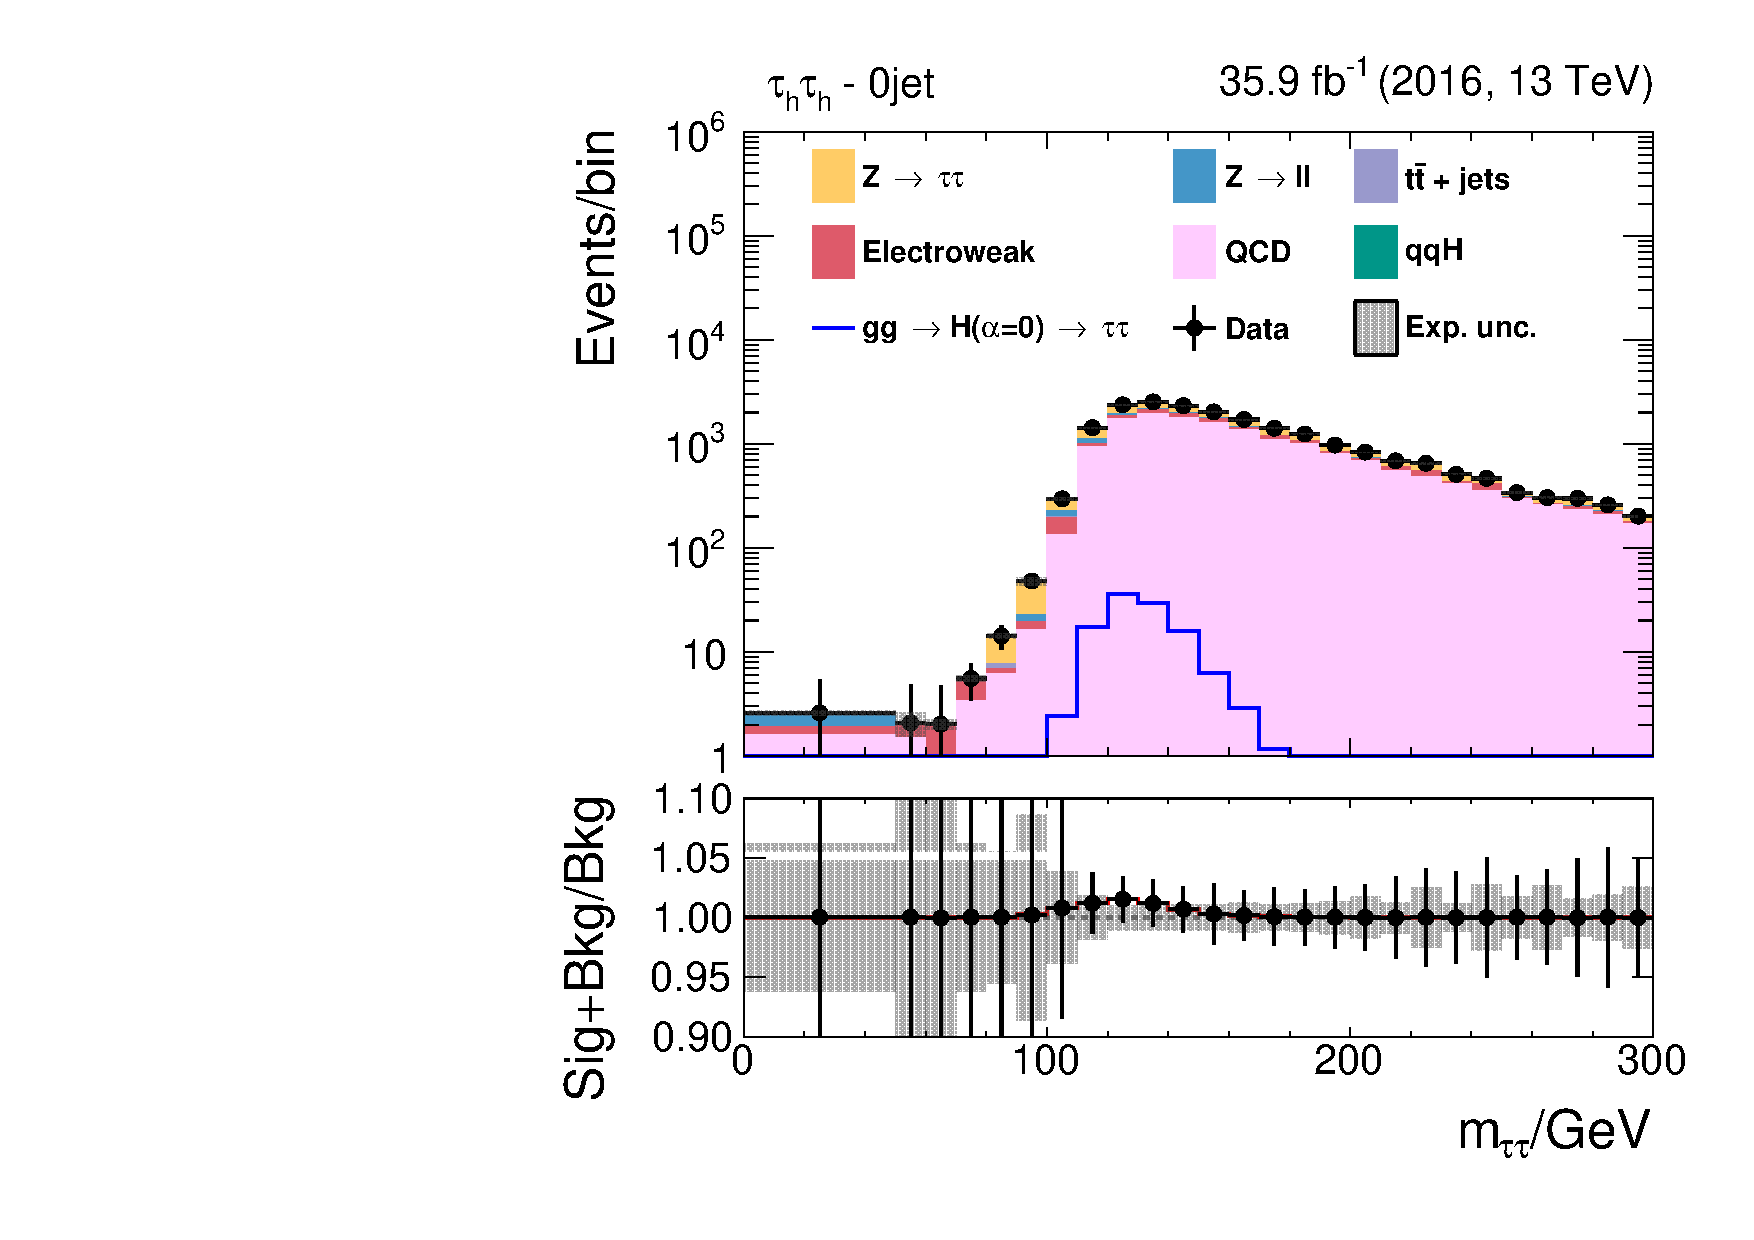
\includegraphics[width=.5\textwidth]{Figures/statana/Postfit_JEC_mela3D/postfit_fit_s_htt_tt_1_13TeV.pdf}
        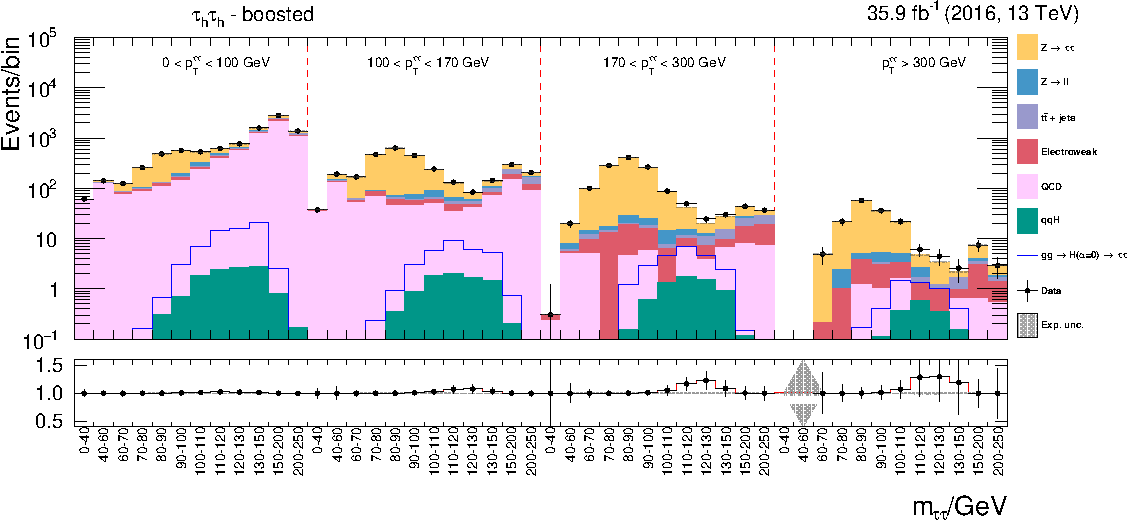
\includegraphics[width=\textwidth]{Figures/statana/Postfit_JEC_mela3D/postfit_fit_s_htt_tt_2_13TeV-crop.pdf}
    \caption[Unrolled postfit distributions in the \textit{0-jet} and \textit{boosted} category in the \tautau{} channel.]{Postfit distributions of the expected background and signal model and pseudo-data with signal-plus-background-to-background ratio in the \textit{0-jet} (upper row) and \textit{boosted} (bottom row) categories for the \tautau{} channel.
    For the \textit{boosted} category the unrolled 2D histogram is shown. First, the distribution is unrolled in bins of \ptautau{} and then along \msv. The 
        borders between bins of \ptautau are indicated through the red dashed lines.}\label{SA:tt_postfit_0jet_1jet}
\end{figure}% 

\begin{figure}[h!]
    \centering 
        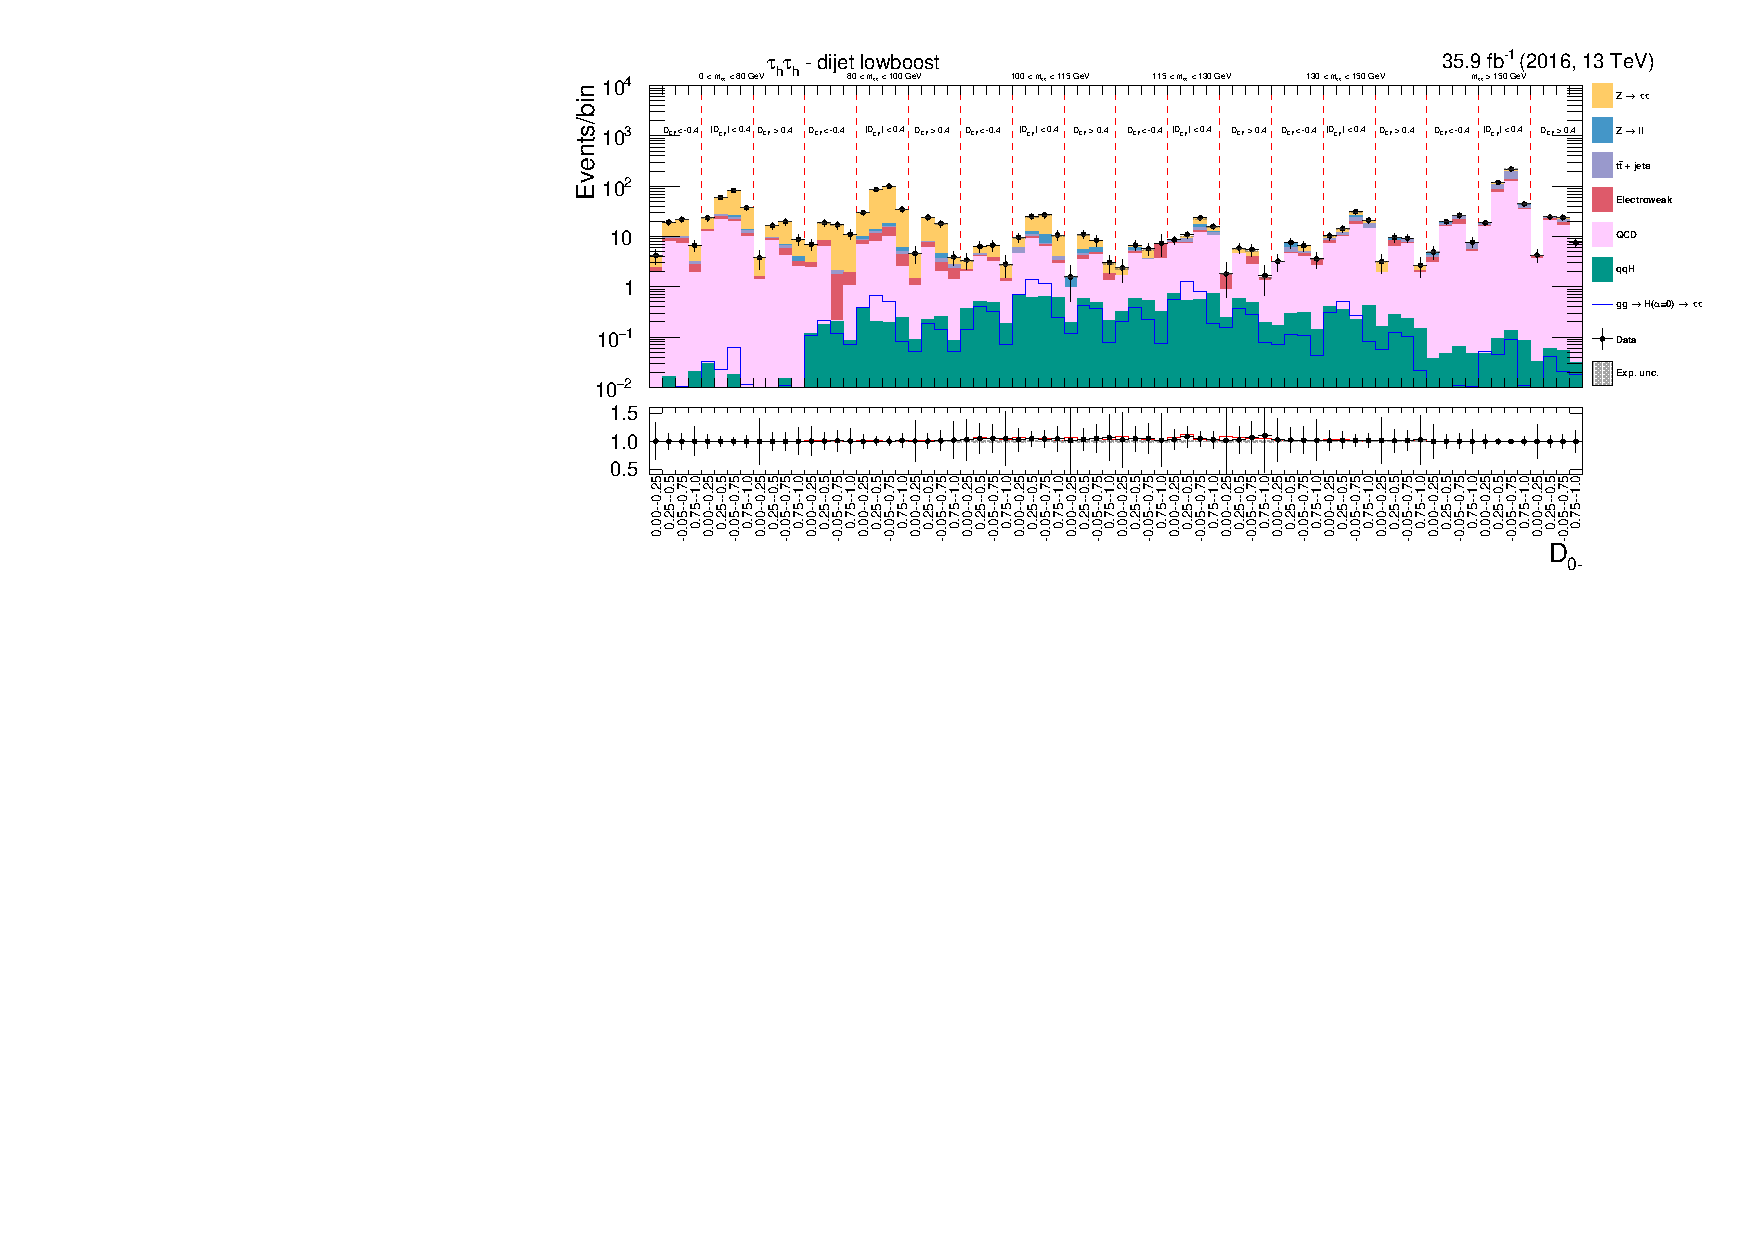
\includegraphics[width=\textwidth]{Figures/statana/Postfit_JEC_mela3D/postfit_fit_s_htt_tt_3_13TeV.pdf}
        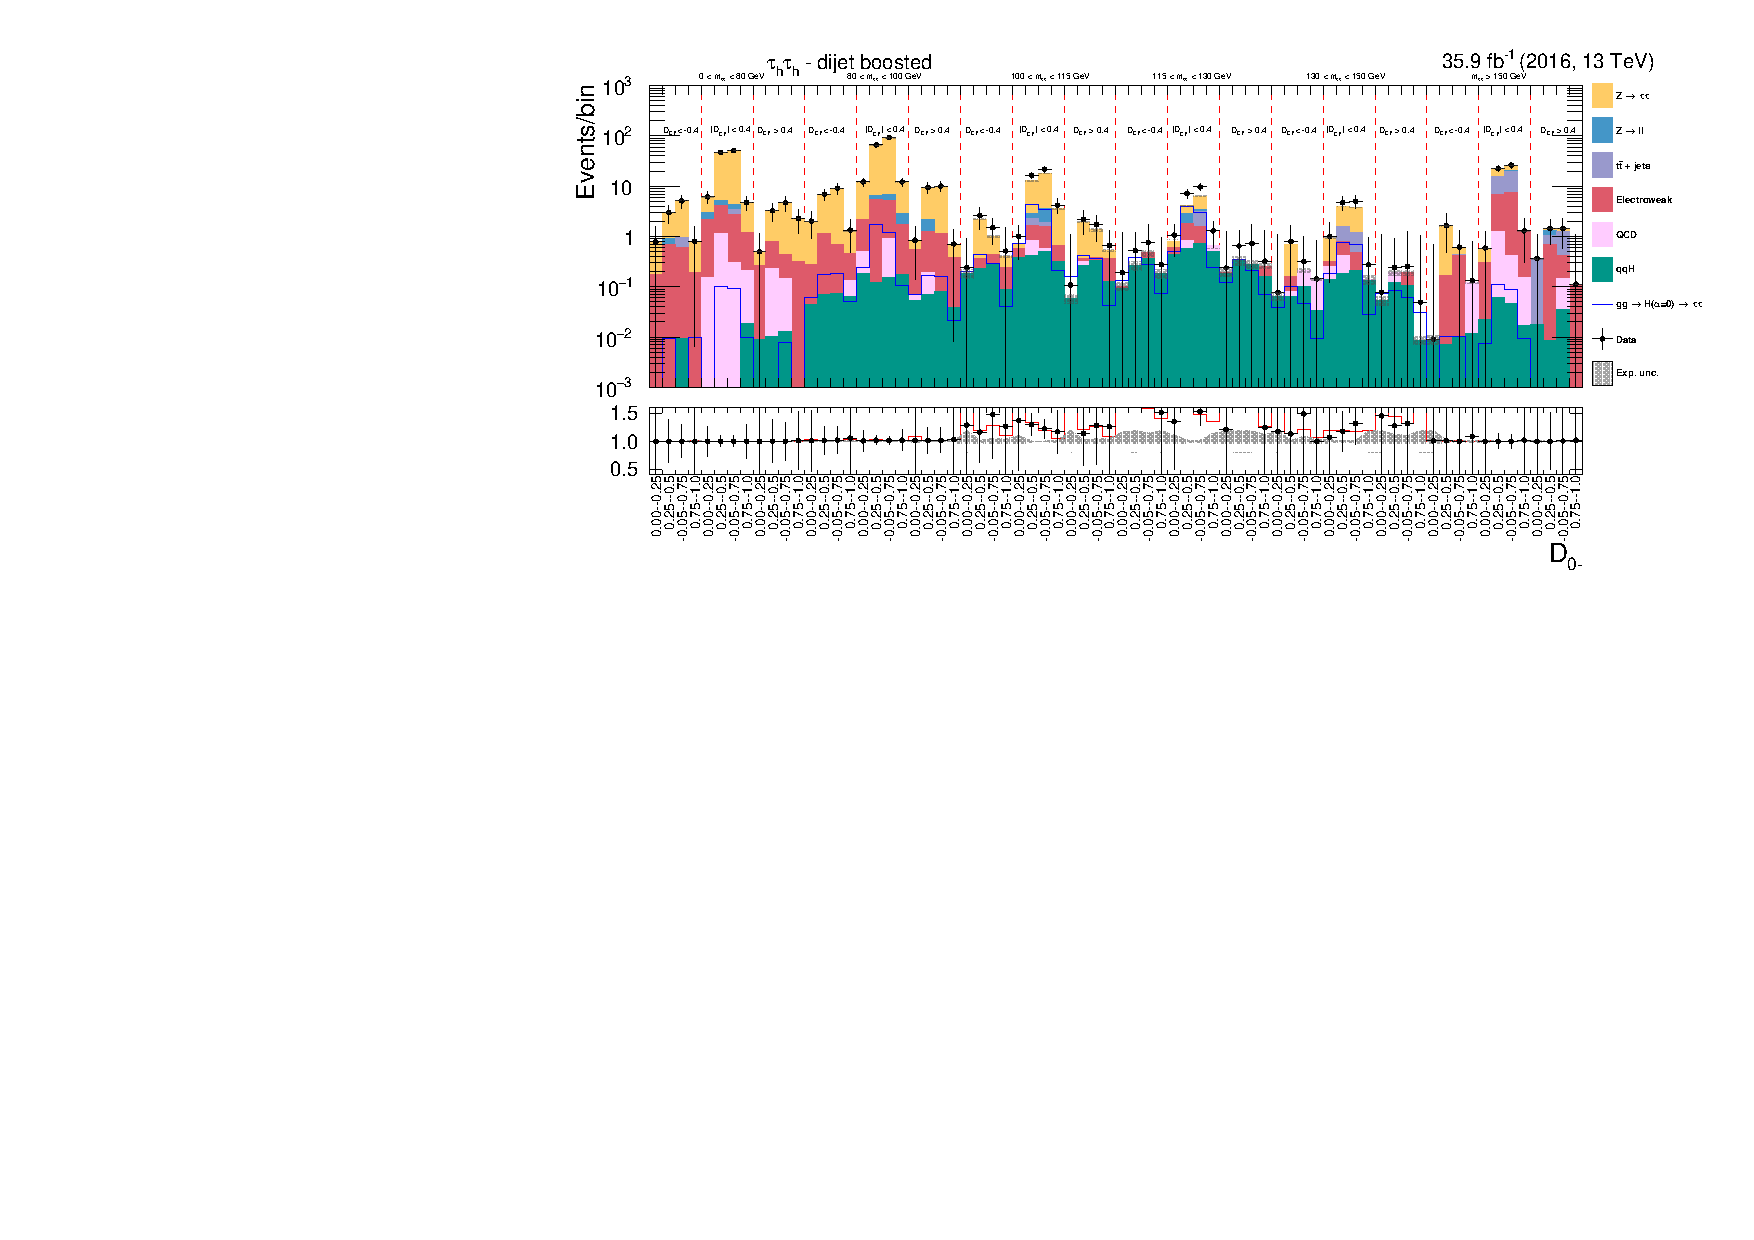
\includegraphics[width=\textwidth]{Figures/statana/Postfit_JEC_mela3D/postfit_fit_s_htt_tt_4_13TeV.pdf}     
    \caption[Unrolled postfit distributions in the \textit{dijet lowboost} and \textit{dijet boosted} category in the \tautau{} channel.]{Postfit distributions of the expected background and signal model and pseudo-data with signal+background to background ratio in the \textit{dijet lowboost} (upper row) and \textit{dijet boosted} (bottom row) categories for the \tautau{} channel.
    The 3D histogram is unrolled first along \msv, then along $D_\text{CP}$ and finally along $D_{0-}$. The borders between neighboring bins of $D_\text{CP}$ are indicated by the red dashed lines. Bins of \msv{} are indicated by on top of the frame and belong always to three bins of $D_\text{CP}$.
    In the bottom plot it is possbile to see that the signal-to-background ratio is optimal in bins of \msv{} that are close to the Higgs boson mass of $\text{125.18\,GeV}$. }\label{SA:tt_postfit_2jet}
\end{figure}%

\subsection{Results}
% Scans for alpha with SM VBF - both single scan and channel comparison
% python $CMSSW_BASE/src/CombineHarvester/HTTSMCP2016/scripts/plot1DScan.py --main="$CMSSW_BASE/src/CombineHarvester/HTTSMCP2016/output/2018-09-23_FULL_mela3D_JECgroupings/cmb/125/higgsCombine.alpha.MultiDimFit.mH125.root" --POI=alpha --output="CombineHarvester/HTTSMCP2016/output/2018-09-23_FULL_mela3D_JECgroupings/cmb/125/alpha" --no-numbers  --no-box --x_title='#alpha_{t}(#frac{#pi}{2})' --y-max=3.0 --use-html-colors --title="#alpha_{t}"
% python $CMSSW_BASE/src/CombineHarvester/HTTSMCP2016/scripts/plot1DScan.py --main=CombineHarvester/HTTSMCP2016/output/2018-09-23_FULL_mela3D_JECgroupings/cmb/125/higgsCombine.alpha.MultiDimFit.mH125.root --POI=alpha --output=CombineHarvester/HTTSMCP2016/output/2018-09-23_FULL_mela3D_JECgroupings/cmb/125/alpha_channel --no-numbers --no-box --x_title='#alpha (#frac{#pi}{2})' --y-max=3.0 --others CombineHarvester/HTTSMCP2016/output/2018-09-23_FULL_mela3D_JECgroupings/tt/125/higgsCombine.alpha.MultiDimFit.mH125.root:#tau_{h}#tau_{h}:#FF5722 CombineHarvester/HTTSMCP2016/output/2018-09-23_FULL_mela3D_JECgroupings/mt/125/higgsCombine.alpha.MultiDimFit.mH125.root:#mu#tau_{h}:#4CAF50 CombineHarvester/HTTSMCP2016/output/2018-09-23_FULL_mela3D_JECgroupings/et/125/higgsCombine.alpha.MultiDimFit.mH125.root:e#tau_{h}:#CDDC39 CombineHarvester/HTTSMCP2016/output/2018-09-23_FULL_mela3D_JECgroupings/em/125/higgsCombine.alpha.MultiDimFit.mH125.root:e#mu:#FFC107 --use-html-colors

% Uncertainty breakdown plot
% python /afs/desy.de/user/d/dwolfsch/cms_analysis/CMSSW_8_1_0/src/CombineHarvester/HTTSMCP2016/scripts/plot1DScan.py --main=CombineHarvester/HTTSMCP2016/output/2018-09-23_FULL_mela3D_JECgroupings/cmb/125/higgsCombine.alpha.MultiDimFit.mH125.root --others 'CombineHarvester/HTTSMCP2016/output/2018-09-23_FULL_mela3D_JECgroupings/cmb/125/higgsCombine.alpha_stat.MultiDimFit.mH125.root:W/O Syst.Unc.:#FF5722' --breakdown syst,stat --use-html-colors --POI=alpha --output="CombineHarvester/HTTSMCP2016/output/2018-09-23_FULL_mela3D_JECgroupings/cmb/125/alpha_breakdown" --x_title='#alpha_{t}(#frac{#pi}{2})' --y-max=5.0

Figure \ref{statana:scan_alpha_f0} shows the expected performance of the measurement of the CP mixing angle $\alpha$ using the kinematic observables $D_\text{CP}$ and $D_{0-}$. 
To perform a pure shape analysis, the signal strength parameters $\mu_\text{F}$ and $\mu_\text{V}$ are 
left floating in the fit. The VBF background is assumed to be SM-like by fixing $f=0$ in the fit. Including all systematic uncertainties and control regions, the analysis is able to distinguish 
between a pure scalar and pseudoscalar fermionic coupling at $\text{1.34}\,\sigma$ (right plot in \figreft{statana:scan_alpha_f0}). The settings of the pseudo-data set are found by measuring \alpha{} with an accuracy of $\text{41}\degree$, which is read off the $1\,\sigma$ band. Examining the performance in the individual decay channels (middle plot in  \figreft{statana:scan_alpha_f0})
one observes the \tautau{} channel to provide the best performance to discriminate between different CP scenarios. As expected the $e\mu$ final state yields the worst performance because it has the smallest signal-to-background ratio \figref{SUPPLE:SA:postfit_em_2jet}.
In order to see whether the fit is capable of reconstructing the imposed signal strength of the pseudo-data set, $\mu_\text{F}$ was profiled with the same setup leaving $\alpha$ floating in the fit.
 As can be seen in \figreft{statana:scan_muF_f0}, the fit is able to find the correct signal strength of $\mu_\text{F}=1$ in all channels. Here, the measurement comes with an uncertainty of $0.5$ for the optimal discriminators. 
% combineTool.py -m 125 -M MultiDimFit --setParameters muF=1,muV=1,alpha=0,f=0 --freezeParameters f --setParameterRanges alpha=0,1 --points 20 --redefineSignalPOIs alpha -d /afs/desy.de/user/d/dwolfsch/cms_analysis/CMSSW_8_1_0/src/CombineHarvester/HTTSMCP2016/output/2018-09-23_FULL_mela3D_JECgroupings/{cmb,em,et,mt,tt}/125/ws.root --algo grid -t -1 --there -n .alpha --parallel=10

% combineTool.py -m 125 -M MultiDimFit --setParameters muF=1,muV=1,alpha=0,f=0 --freezeParameters f --setParameterRanges alpha=0,1 --points 20  --redefineSignalPOIs alpha -d /afs/desy.de/user/d/dwolfsch/cms_analysis/CMSSW_8_1_0/src/CombineHarvester/HTTSMCP2016/output/2018-09-23_FULL_jdphi_JECgroupings_no_2jet_cr/{cmb,em,et,mt,tt}/125/ws.root --algo grid -t -1 --there -n .alpha --parallel=10
\begin{figure}[h!]
    \centering
    \begin{subfigure}{.49\textwidth}
        \centering
        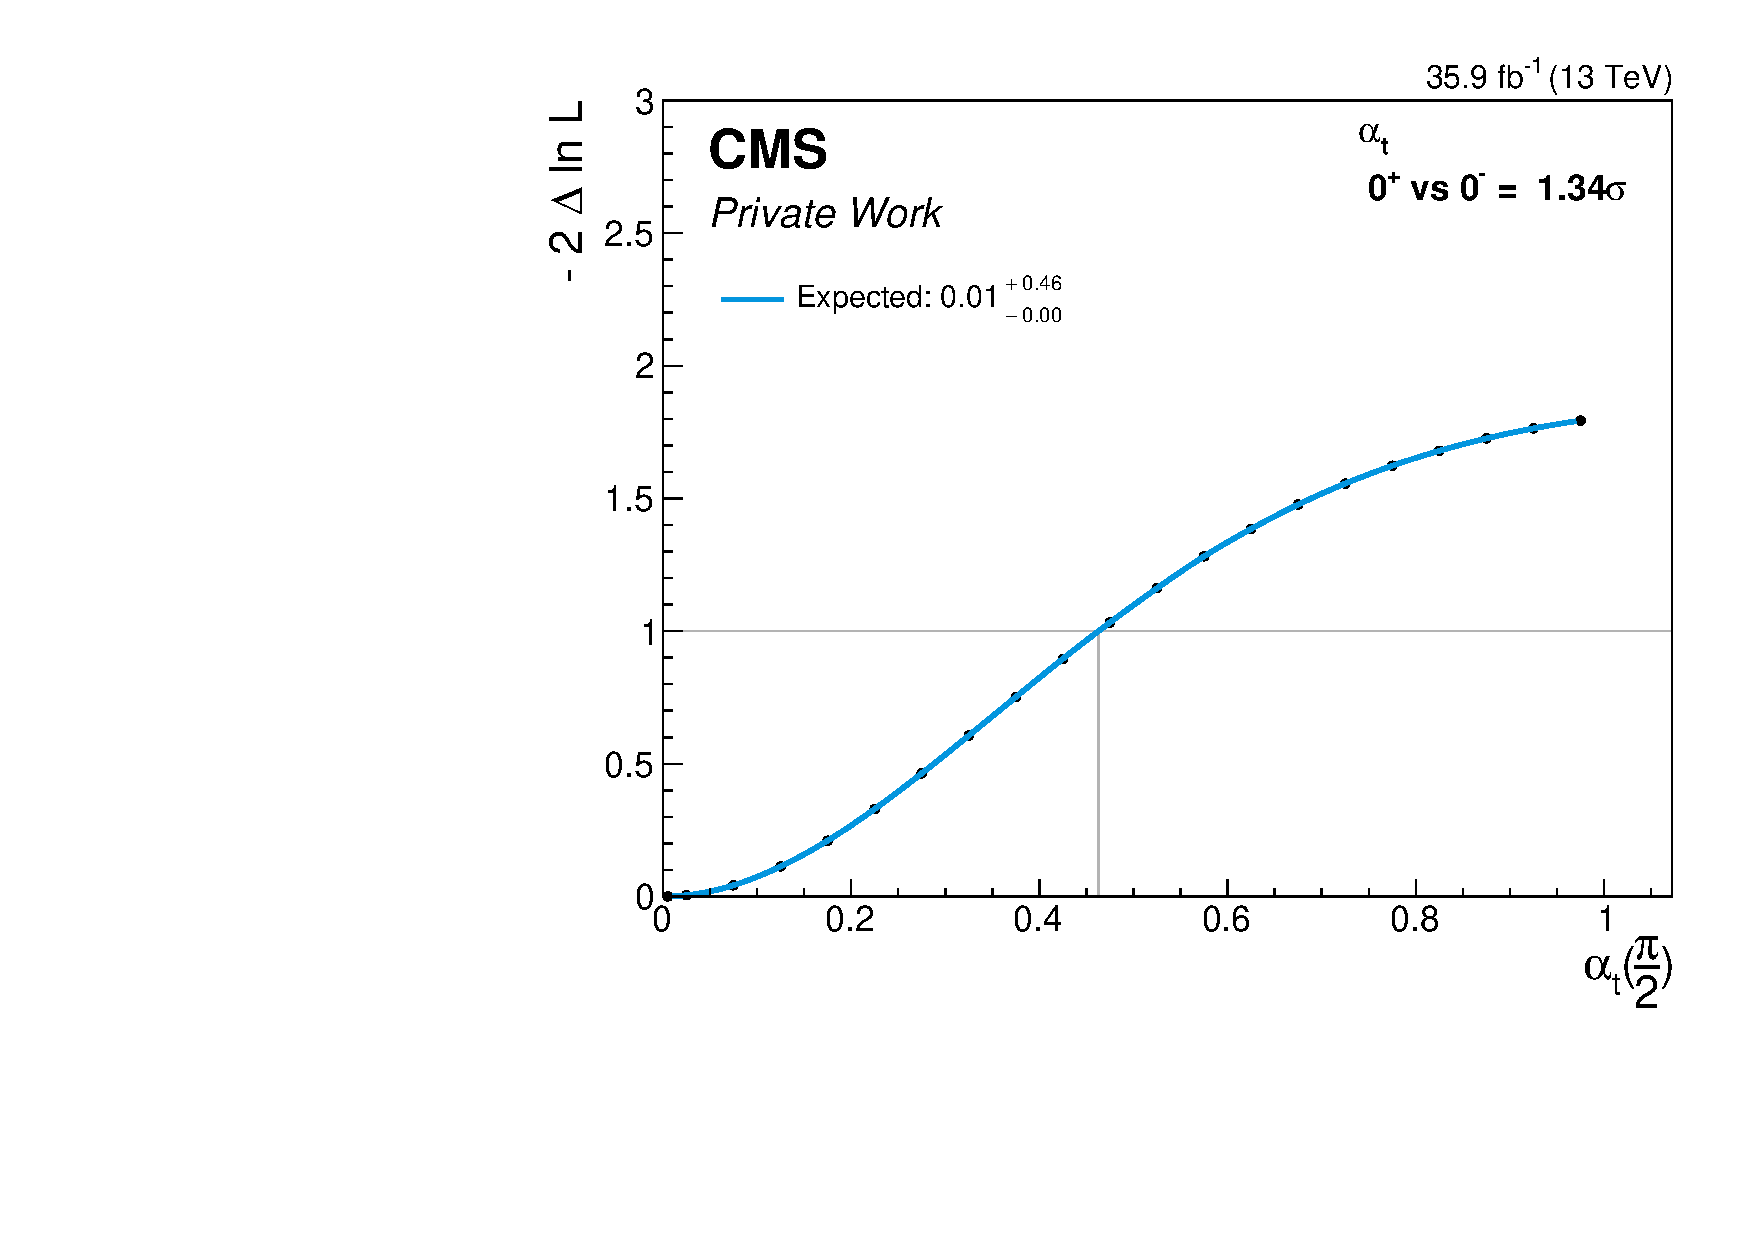
\includegraphics[width=\textwidth]{Figures/statana/Scan_JEC_mela3D/alpha.pdf}
    \end{subfigure}
    \begin{subfigure}{.49\textwidth}
        \centering
        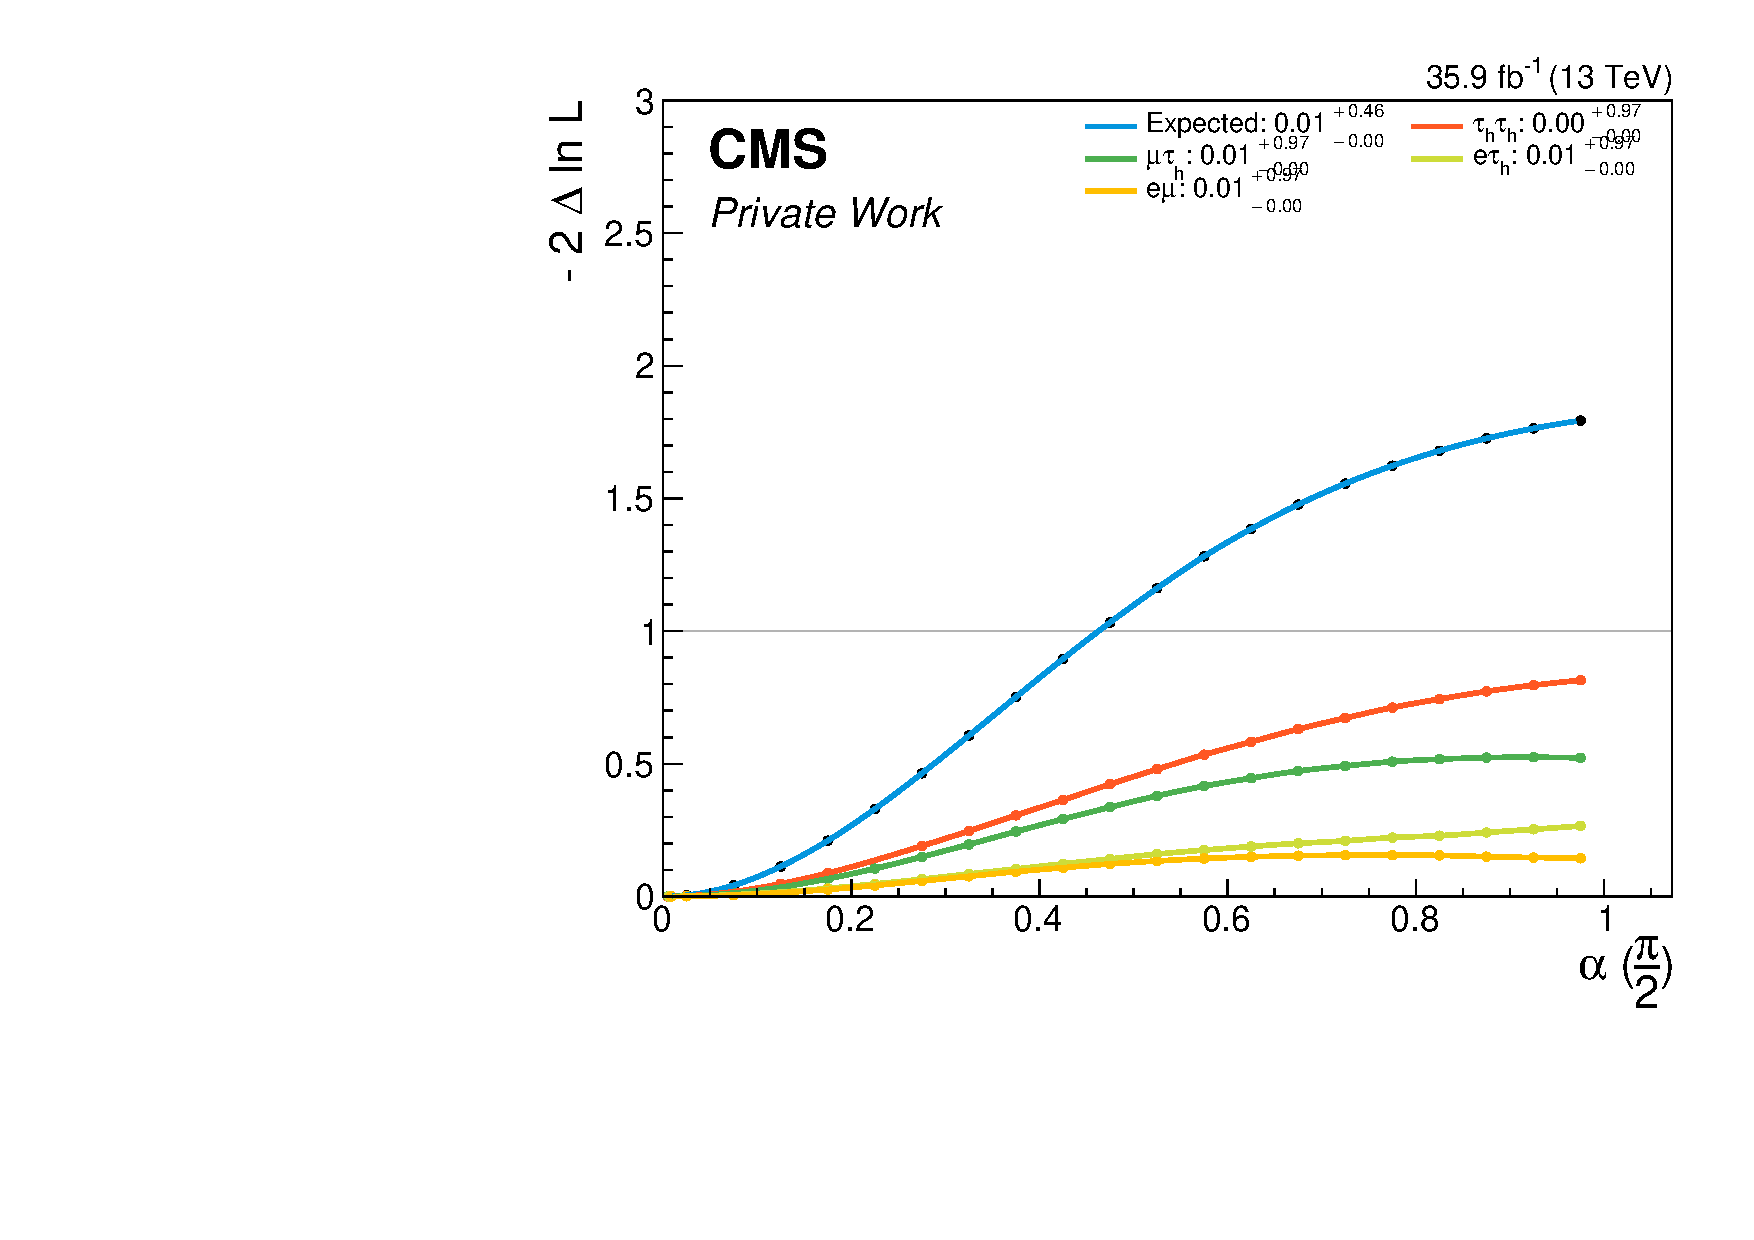
\includegraphics[width=\textwidth]{Figures/statana/Scan_JEC_mela3D/alpha_channel.pdf}
    \end{subfigure}
    \caption[Measurement of $\alpha$ with channel comparison using the MELA observables.]{Measurement of the CP mixing angle $\alpha$ in the fermionic couplings of the Higgs boson to the top quark inferred from the effective gluon coupling under the assumption of a scalar Higgs boson and SM-like VBF production ($f=0$). The analysis is able to distinguish a scalar from a pseudoscalar CP scenario using the MELA approach at $\text{1.34\,\sigma}$.
    The right plot shows the measurement in each individual decay channel. The \tautau{} channel is the most significant channel followed by the 
    \mutau{} channel.}\label{statana:scan_alpha_f0}
\end{figure}

% MELA muF scans 
% combineTool.py -m 125 -M MultiDimFit --setParameters muF=1,muV=1,alpha=0,f=0 --freezeParameters f --setParameterRanges muF=0,4 --points 20  --redefineSignalPOIs muF -d /afs/desy.de/user/d/dwolfsch/cms_analysis/CMSSW_8_1_0/src/CombineHarvester/HTTSMCP2016/output/2018-09-23_FULL_mela3D_JECgroupings/{cmb,em,et,mt,tt}/125/ws.root --algo grid -t -1 --there -n .muF --parallel=10
% python $CMSSW_BASE/src/CombineHarvester/HTTSMCP2016/scripts/plot1DScan.py --main="$CMSSW_BASE/src/CombineHarvester/HTTSMCP2016/output/2018-09-23_FULL_mela3D_JECgroupings/cmb/125/higgsCombine.muF.MultiDimFit.mH125.root" --POI=muF --output="CombineHarvester/HTTSMCP2016/output/2018-09-23_FULL_mela3D_JECgroupings/cmb/125/muF" --no-numbers  --no-box --x_title='#mu_{F}' --y-max=10.0 --use-html-colors --title="#mu_{F}(f=0)"
% python $CMSSW_BASE/src/CombineHarvester/HTTSMCP2016/scripts/plot1DScan.py --main=CombineHarvester/HTTSMCP2016/output/2018-09-23_FULL_mela3D_JECgroupings/cmb/125/higgsCombine.muF.MultiDimFit.mH125.root --POI=muF --output=CombineHarvester/HTTSMCP2016/output/2018-09-23_FULL_mela3D_JECgroupings/cmb/125/muF_channel --no-numbers --no-box --x_title='#mu_{F}' --y-max=12.0 --others CombineHarvester/HTTSMCP2016/output/2018-09-23_FULL_mela3D_JECgroupings/tt/125/higgsCombine.muF.MultiDimFit.mH125.root:#tau_{h}#tau_{h}:#FF5722 CombineHarvester/HTTSMCP2016/output/2018-09-23_FULL_mela3D_JECgroupings/mt/125/higgsCombine.muF.MultiDimFit.mH125.root:#mu#tau_{h}:#4CAF50 CombineHarvester/HTTSMCP2016/output/2018-09-23_FULL_mela3D_JECgroupings/et/125/higgsCombine.muF.MultiDimFit.mH125.root:e#tau_{h}:#CDDC39 CombineHarvester/HTTSMCP2016/output/2018-09-23_FULL_mela3D_JECgroupings/em/125/higgsCombine.muF.MultiDimFit.mH125.root:e#mu:#FFC107 --use-html-colors


% jdphi muF scans
% combineTool.py -m 125 -M MultiDimFit --setParameters muF=1,muV=1,alpha=0,f=0 --freezeParameters f --setParameterRanges muF=0,4 --points 20  --redefineSignalPOIs muF -d /afs/desy.de/user/d/dwolfsch/cms_analysis/CMSSW_8_1_0/src/CombineHarvester/HTTSMCP2016/output/2018-09-23_FULL_jdphi_JECgroupings_no_2jet_cr/{cmb,em,et,mt,tt}/125/ws.root --algo grid -t -1 --there -n .muF --parallel=10
% python $CMSSW_BASE/src/CombineHarvester/HTTSMCP2016/scripts/plot1DScan.py --main="/afs/desy.de/user/d/dwolfsch/cms_analysis/CMSSW_8_1_0/src/CombineHarvester/HTTSMCP2016/output/2018-09-23_FULL_jdphi_JECgroupings_no_2jet_cr/cmb/125/higgsCombine.muF.MultiDimFit.mH125.root" --POI=muF --output="CombineHarvester/HTTSMCP2016/output/2018-09-23_FULL_jdphi_JECgroupings_no_2jet_cr/cmb/125/muF" --no-numbers  --no-box --x_title='#mu_{F}' --y-max=10.0 --use-html-colors --title="#mu_{F}(f=0)"
% python $CMSSW_BASE/src/CombineHarvester/HTTSMCP2016/scripts/plot1DScan.py --main=CombineHarvester/HTTSMCP2016/output/2018-09-23_FULL_jdphi_JECgroupings_no_2jet_cr/cmb/125/higgsCombine.muF.MultiDimFit.mH125.root --POI=muF --output=CombineHarvester/HTTSMCP2016/output/2018-09-23_FULL_jdphi_JECgroupings_no_2jet_cr/cmb/125/muF_channel --no-numbers --no-box --x_title='#mu_{F}' --y-max=12.0 --others CombineHarvester/HTTSMCP2016/output/2018-09-23_FULL_jdphi_JECgroupings_no_2jet_cr/tt/125/higgsCombine.muF.MultiDimFit.mH125.root:#tau_{h}#tau_{h}:#FF5722 CombineHarvester/HTTSMCP2016/output/2018-09-23_FULL_jdphi_JECgroupings_no_2jet_cr/mt/125/higgsCombine.muF.MultiDimFit.mH125.root:#mu#tau_{h}:#4CAF50 CombineHarvester/HTTSMCP2016/output/2018-09-23_FULL_jdphi_JECgroupings_no_2jet_cr/et/125/higgsCombine.muF.MultiDimFit.mH125.root:e#tau_{h}:#CDDC39 CombineHarvester/HTTSMCP2016/output/2018-09-23_FULL_jdphi_JECgroupings_no_2jet_cr/em/125/higgsCombine.muF.MultiDimFit.mH125.root:e#mu:#FFC107 --use-html-colors

\begin{figure}[h!]
    \centering
    \begin{subfigure}{.49\textwidth}
        \centering
        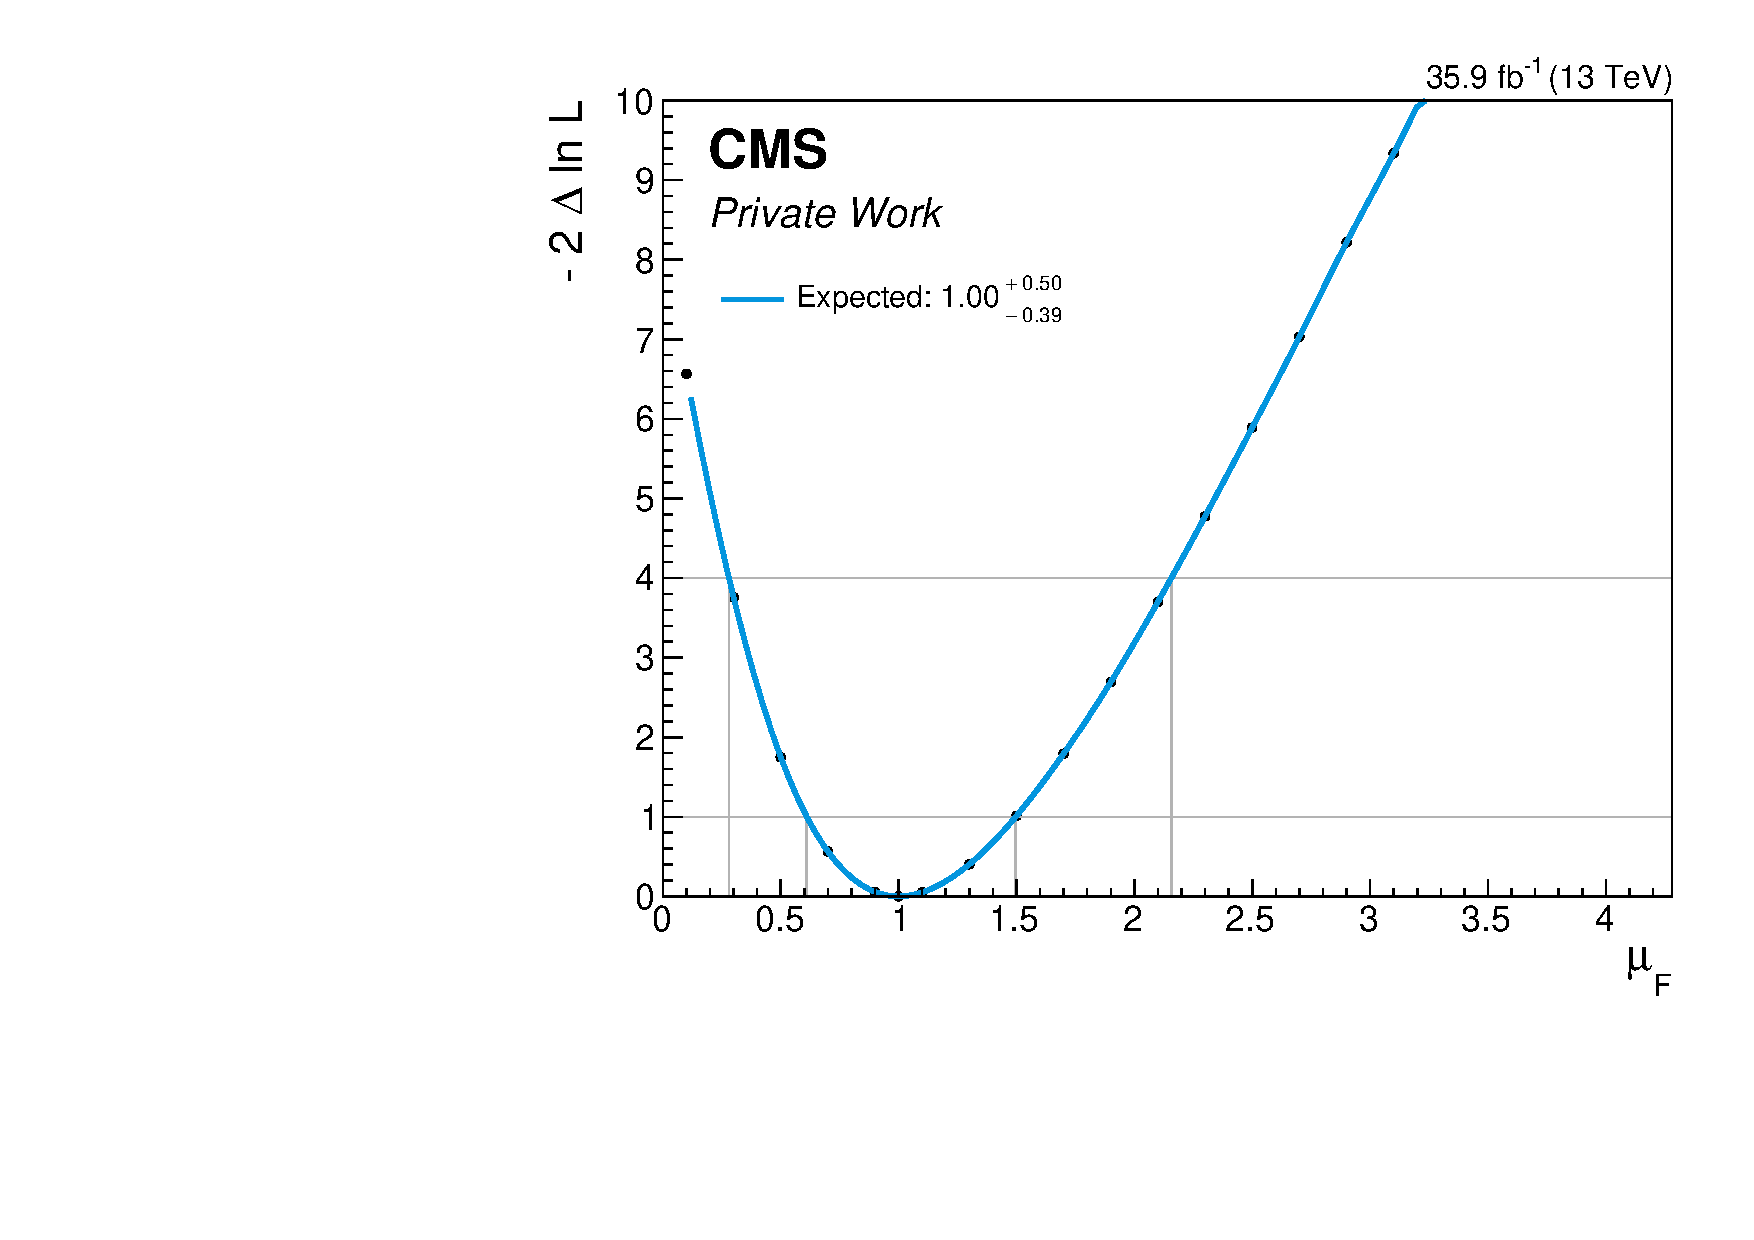
\includegraphics[width=\textwidth]{Figures/statana/Scan_JEC_mela3D/muF.pdf}
    \end{subfigure}
    \begin{subfigure}{.49\textwidth}
        \centering
        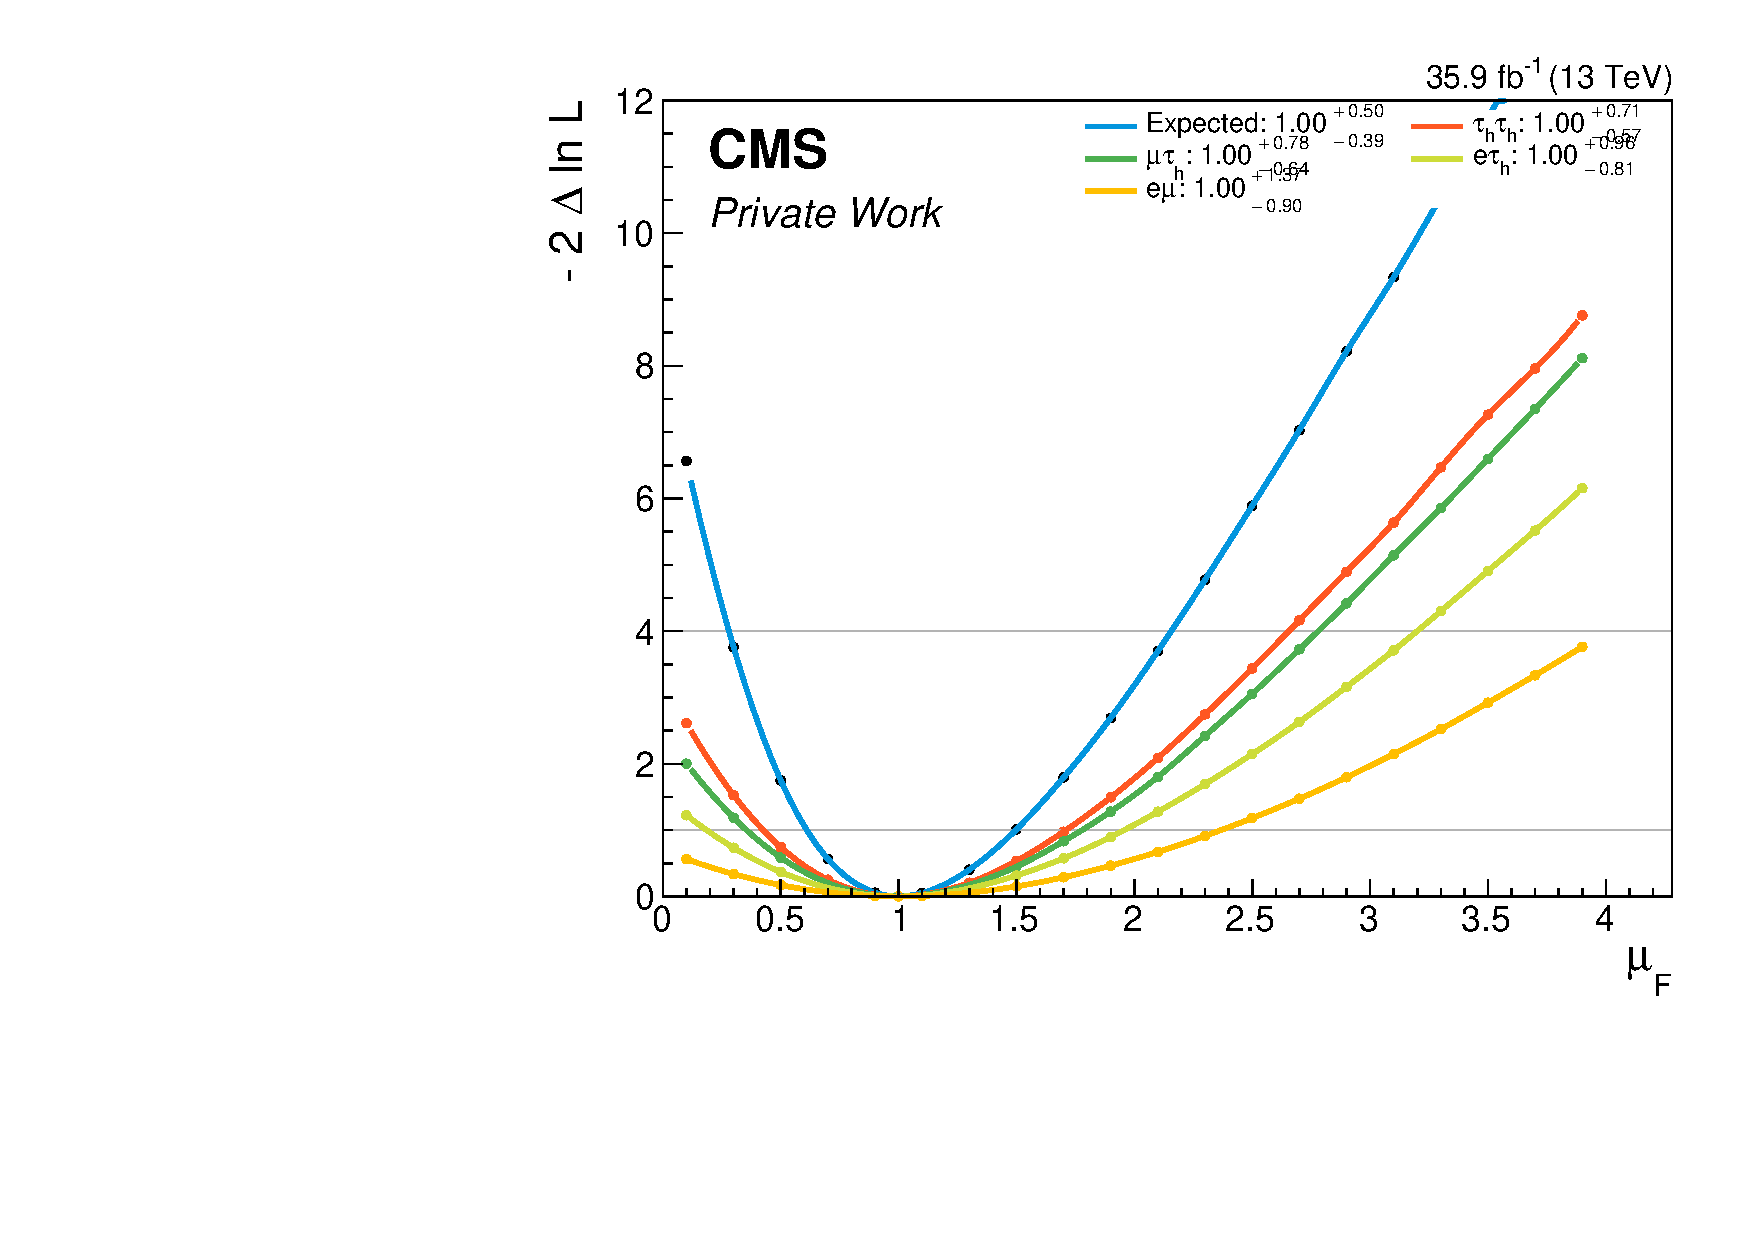
\includegraphics[width=\textwidth]{Figures/statana/Scan_JEC_mela3D/muF_channel.pdf}
    \end{subfigure}
    \caption[Measurement of the signal strength modifier $\mu_\text{F}$ with the MELA approach.]{Measurement of the gluon-gluon fusion signal strength utilizing a signal model assuming a scalar Higgs boson and SM-like VBF production ($f=\text{0}$). The analysis is able to find $\mu_\text{F}$ at the value set by the pseudo-data set with an accuracy of $0.5$.
    The right plot shows the measurement in each individual decay channel. Again the \tautau{} channel yields the tightest constraint followed by the 
    \mutau{} channel. In the left plot the measurement is performed for $\Delta\phi_\text{jj}$ showing that it gives the same result but with a looser constraint only.}\label{statana:scan_muF_f0}
\end{figure}

\subsubsection{Comparison to the measurement using \jdphi{}}
$\alpha$ was also profiled using $\Delta\phi_\text{jj}$ as discriminator instead of the combination of $D_\text{CP}$ and $D_{0-}$. 
The profile is shown in the left plot in \figreft{statana:scan_jdphi}. Using $\Delta\phi_\text{jj}$ as the only discriminant, a less accurate measurement of $\alpha = 0.0^{+45 \degree}_{-0}$ is obtained because the information from four of the five angles in the 
event kinematics is missing. Moreover, this setup is only capable of distinghuishing scalar and pseudoscalar couplings at $\text{1.25\,\sigma}$.
Also here a measurement of the signal strength was performed providing also a less accurate measurement, as depicted in the right plot in \figreft{statana:scan_jdphi}.
The fit uncertainty here yields $0.59$.

 % python $CMSSW_BASE/src/CombineHarvester/HTTSMCP2016/scripts/plot1DScan.py --main=CombineHarvester/HTTSMCP2016/output/2018-09-23_FULL_jdphi_JECgroupings_no_2jet_cr/cmb/125/higgsCombine.alpha.MultiDimFit.mH125.root --POI=alpha --output=CombineHarvester/HTTSMCP2016/output/2018-09-23_FULL_jdphi_JECgroupings_no_2jet_cr/cmb/125/alpha_jdphi --no-numbers --no-box --x_title='#alpha (#frac{#pi}{2})' --y-max=3.0 --others CombineHarvester/HTTSMCP2016/output/2018-09-23_FULL_mela3D_JECgroupings/cmb/125/higgsCombine.alpha.MultiDimFit.mH125.root:MELA:#FF5722 --use-html-colors --title "#Delta#phi_{jj}"
\begin{figure}[h!]
    \centering
    \begin{subfigure}{.49\textwidth}
        \centering
        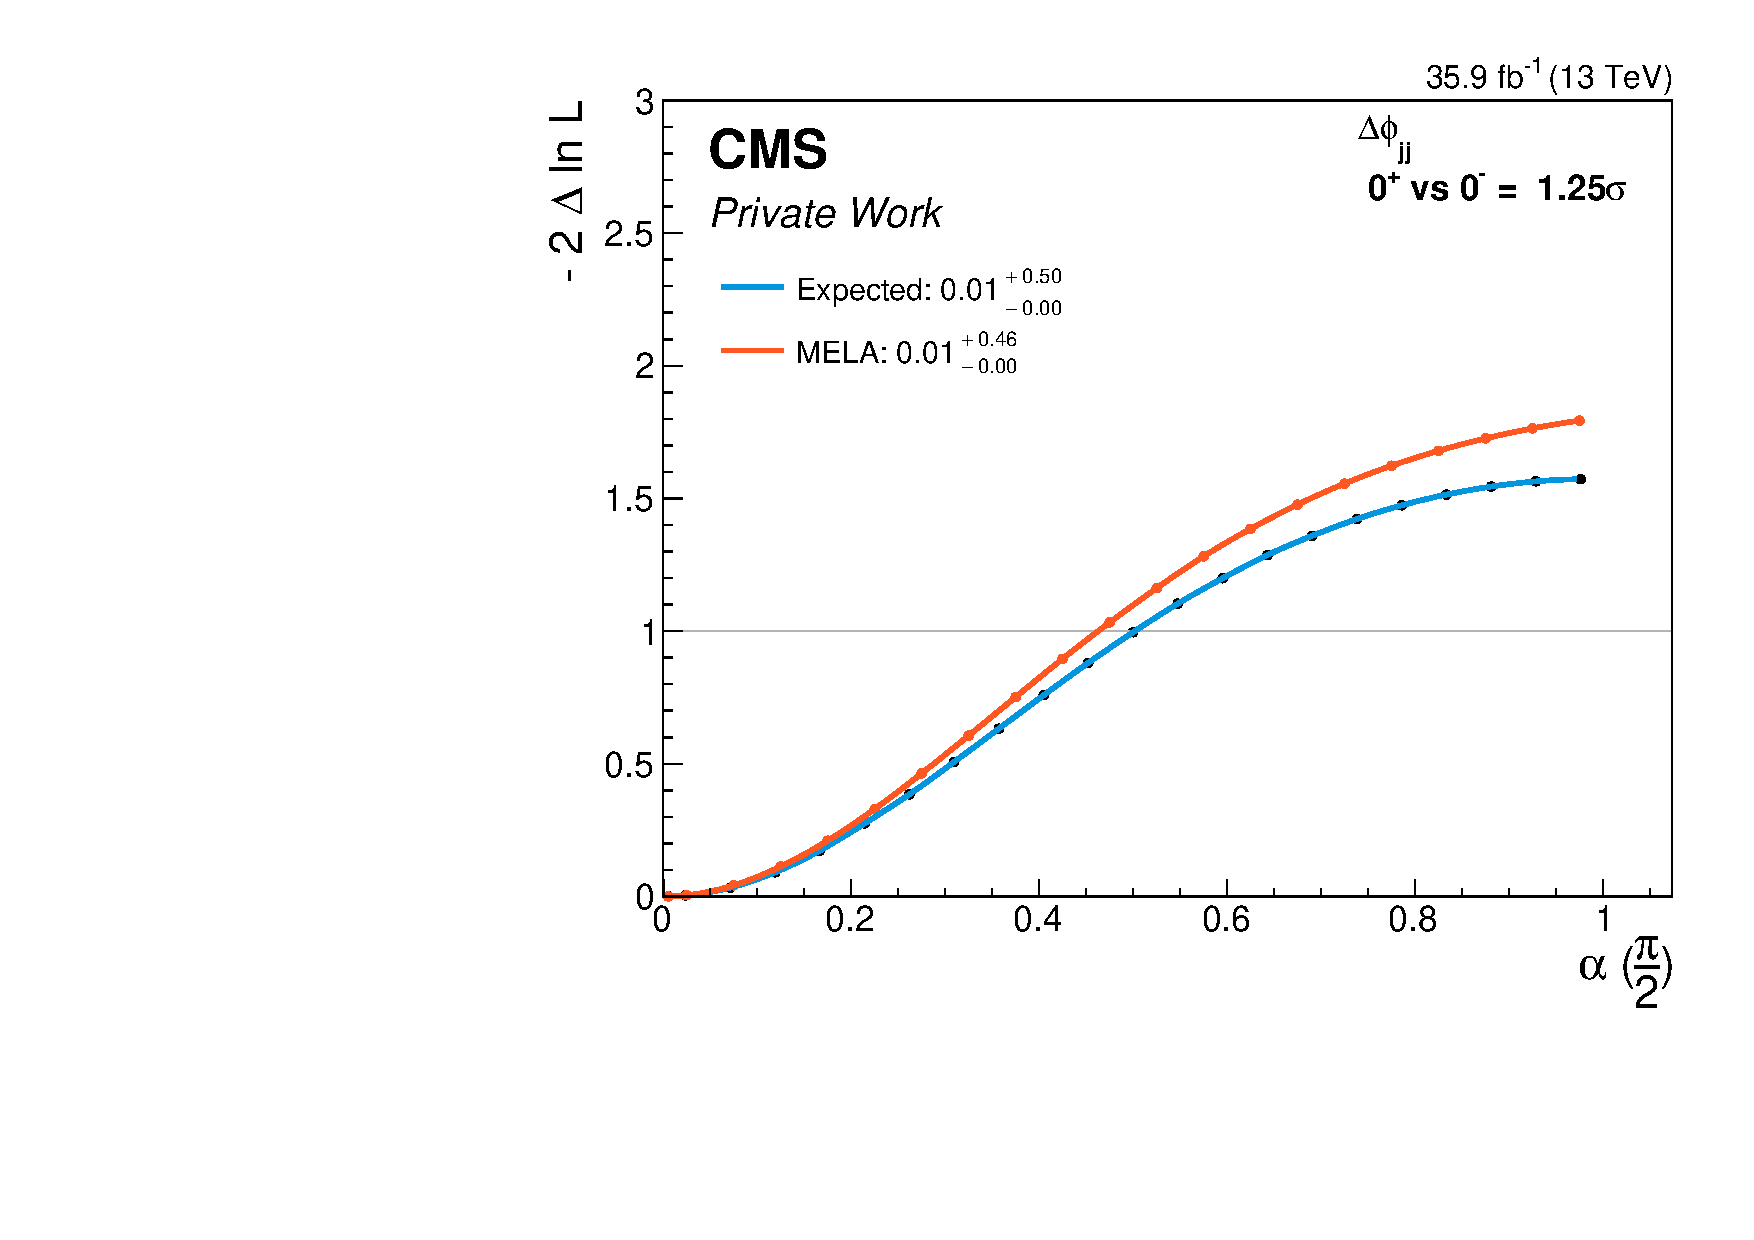
\includegraphics[width=\textwidth]{Figures/statana/Scan_JEC_jdphi/alpha_jdphi.pdf}
    \end{subfigure}
    \begin{subfigure}{.49\textwidth}
        \centering
        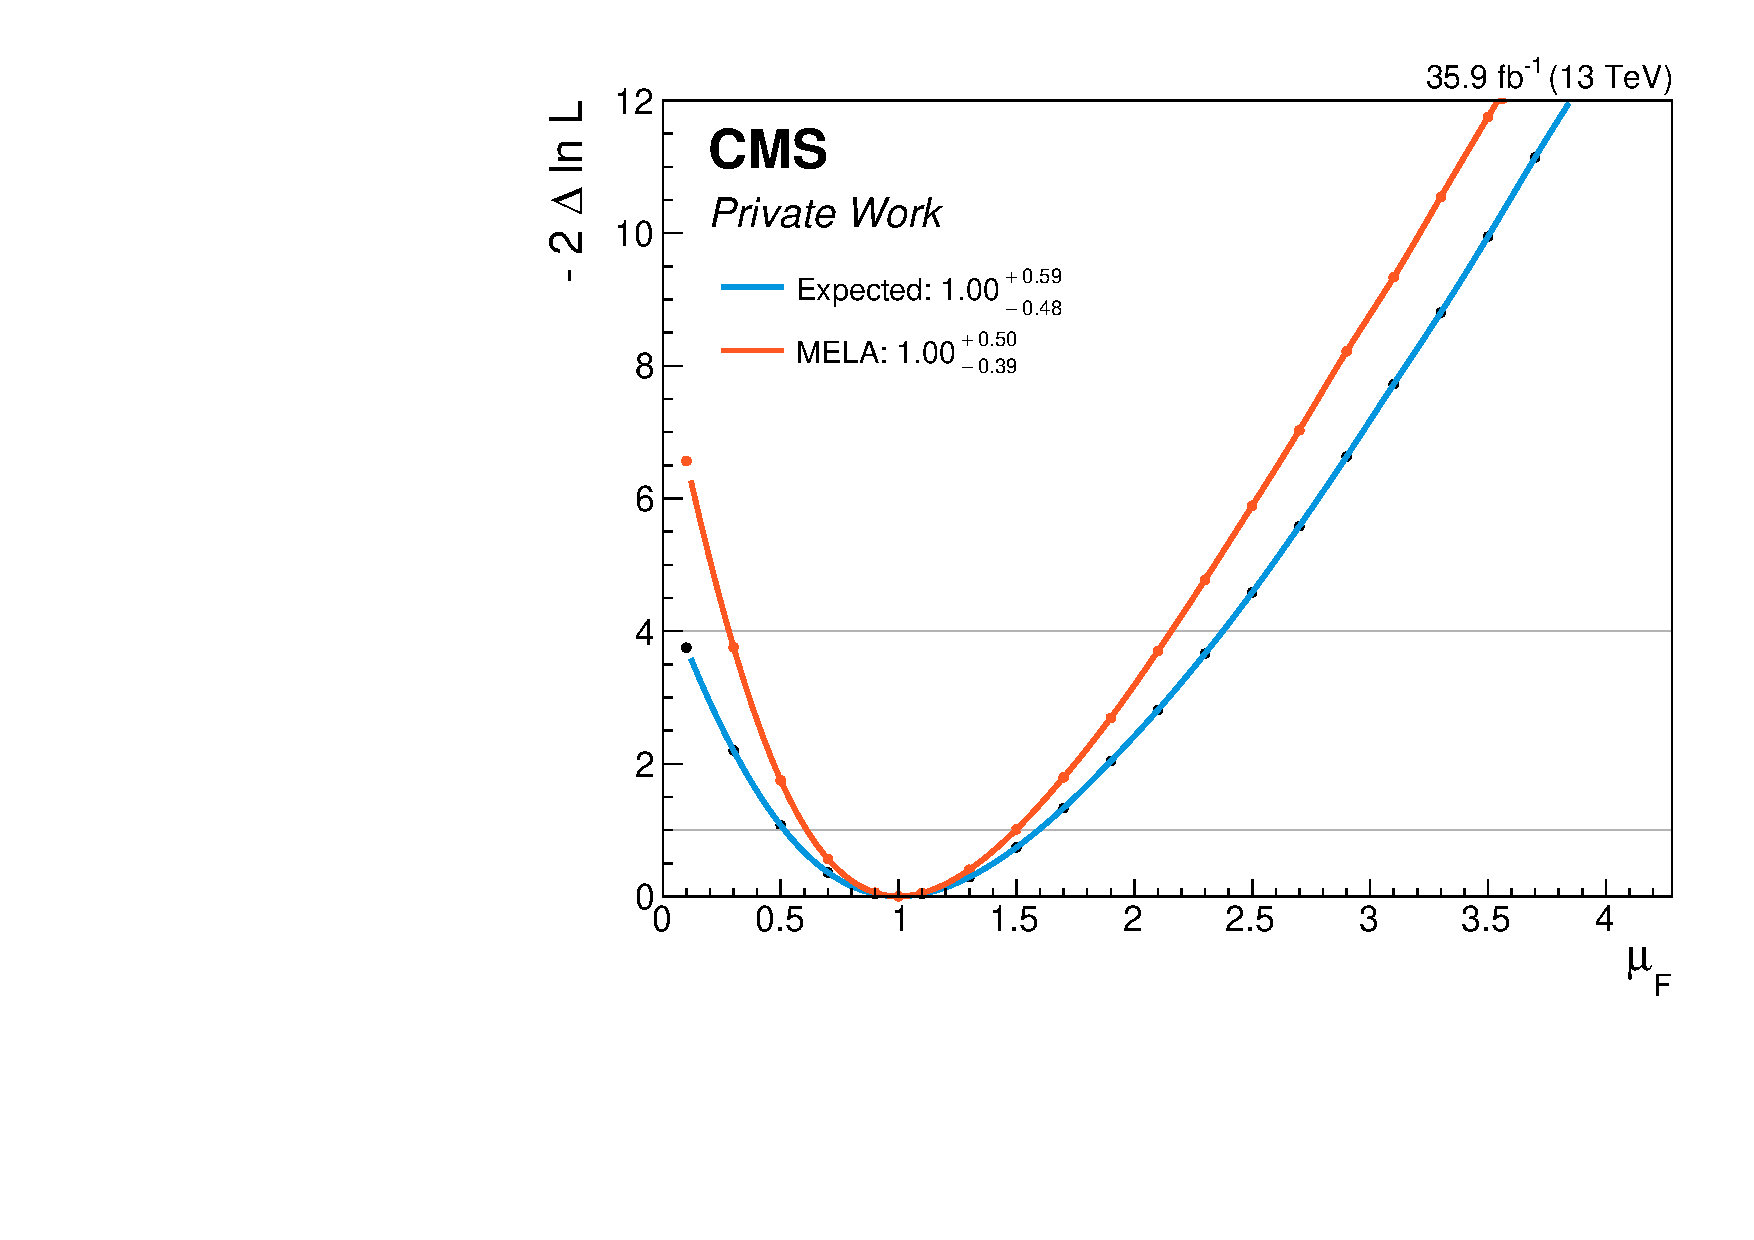
\includegraphics[width=\textwidth]{Figures/statana/Scan_JEC_jdphi/muF_jdphi.pdf}
    \end{subfigure}
    \caption[Measurement of $\alpha$ and $\mu_\text{F}$ using \jdphi{}.]{Measurement of the CP mixing angle $\alpha$ (left) and the signal strength $\mu_\text{F}$ (right) in the fermionic coupling of the Higgs boson to the top quark inferred from the effective gluon coupling under the assumption of a scalar Higgs boson and SM-like VBF production ($f=0$). As shown in the left figure, the analysis is able to distinguish a scalar from a pseudoscalar CP scenario using approach utilizing \jdphi{} (blue) at $\text{1.25\,\sigma}$.
    A lower performance is obtained than with the full angular information taken into account by the MELA approach (orange).
    In the left plot the measurement is performed for $\Delta\phi_\text{jj}$ showing that it gives the same result but with a looser constraint only. The right plot shows the measurement of the signal strength modifier $\mu_\text{F}$ and also shows a larger fit uncertainty. }\label{statana:scan_jdphi}
\end{figure}

\subsubsection{Impact of CP violation in VBF and SM rate constraint}
To study whether the CP state realized in the VBF background has any impact on the performance of the analysis, $\alpha$ is profiled leaving the VBF CP parameter $f$ floating. The result is given in the left
plot in \figreft{statana:scan_alpha_ggF_VBF} showing that the performance is not affected by letting the fit find a best-fit value for $f$ as no change in the fit result is found compared to \figreft{statana:scan_alpha_f0}. This implies that the analysis setup is currently not sensitive to the possible higher-order effects from the VBF CP scenario. 
The reason for this are both that the yield is smaller compared to ggF events in the signal categories and that the effect of a pseudoscalar admixture does not enter at tree level but is suppressed by a loop.
As a consequence, fixing $f=0$ during the measurement of $\alpha$ is a justified approximation.\newline{}
With the signal model introduced above, the rate of the processes and their shapes, that provides the information about the pseudoscalar admixture, can be altered independently from each other. Therefore, the shape analysis performed in this thesis
 gives the most unbiased measurement of $\alpha$. Any effect that also modifies the rate of the ggF process can be due to other physics scenarios such as heavy BSM fermions running in the loop between
the gluons and the Higgs boson instead of a top quark and lighter SM fermions. For this reason, a measurement of $\alpha$ constraining the ggF rate to the known SM value of $\mu_\text{F}=1$ comes with the model-dependent assumption that 
there are no other BSM effects present in the coupling. The impact of fixing $\mu_\text{F}=1$ is examined in the right plot in \figreft{statana:scan_alpha_ggF_VBF}. The model-dependent measurement of $\alpha$ leads to a significantly better precision 
of $\text{24.3}\degree$. Using the constraint the analysis setup can distinguish between a scalar and a pseudoscalar Higgs boson fermionic coupling at $\text{3.65\,\sigma}$. The reason for this is the increased coupling constant of the pseudoscalar coupling in equation \eqref{SA:rate_constraint} expected by the signal model in this case.

% combineTool.py -m 125 -M MultiDimFit --setParameters muF=1,muV=1,alpha=0,f=0 --setParameterRanges alpha=0,1 --points 20 --redefineSignalPOIs alpha -d /afs/desy.de/user/d/dwolfsch/cms_analysis/CMSSW_8_1_0/src/CombineHarvester/HTTSMCP2016/output/2018-09-23_FULL_mela3D_JECgroupings/{cmb,em,et,mt,tt}/125/ws.root --algo grid -t -1 --there -n .alpha_f_floating --parallel=10
% python $CMSSW_BASE/src/CombineHarvester/HTTSMCP2016/scripts/plot1DScan.py --main="/afs/desy.de/user/d/dwolfsch/cms_analysis/CMSSW_8_1_0/src/CombineHarvester/HTTSMCP2016/output/2018-09-23_FULL_mela3D_JECgroupings/cmb/125/higgsCombine.alpha_ggFconstrain.MultiDimFit.mH125.root" --POI=alpha --output="CombineHarvester/HTTSMCP2016/output/2018-09-23_FULL_mela3D_JECgroupings/cmb/125/alpha_ggFconstrain" --no-numbers  --no-box --x_title='#alpha_{t}(#frac{#pi}{2})' --y-max=17.0 --use-html-colors --title="#alpha_{t}(#mu_F=1)"
%  python $CMSSW_BASE/src/CombineHarvester/HTTSMCP2016/scripts/plot1DScan.py --main="$CMSSW_BASE/src/CombineHarvester/HTTSMCP2016/output/2018-09-23_FULL_mela3D_JECgroupings/cmb/125/higgsCombine.alpha_f_floating.MultiDimFit.mH125.root" --POI=alpha --output="CombineHarvester/HTTSMCP2016/output/2018-09-23_FULL_mela3D_JECgroupings/cmb/125/alpha_VBFfloating" --no-numbers  --no-box --x_title='#alpha_{t}(#frac{#pi}{2})' --y-max=3.0 --use-html-colors --title="#alpha_{t}(VBF floating)"
\begin{figure}[h!]
    \centering
    \begin{subfigure}{.49\textwidth}
        \centering
        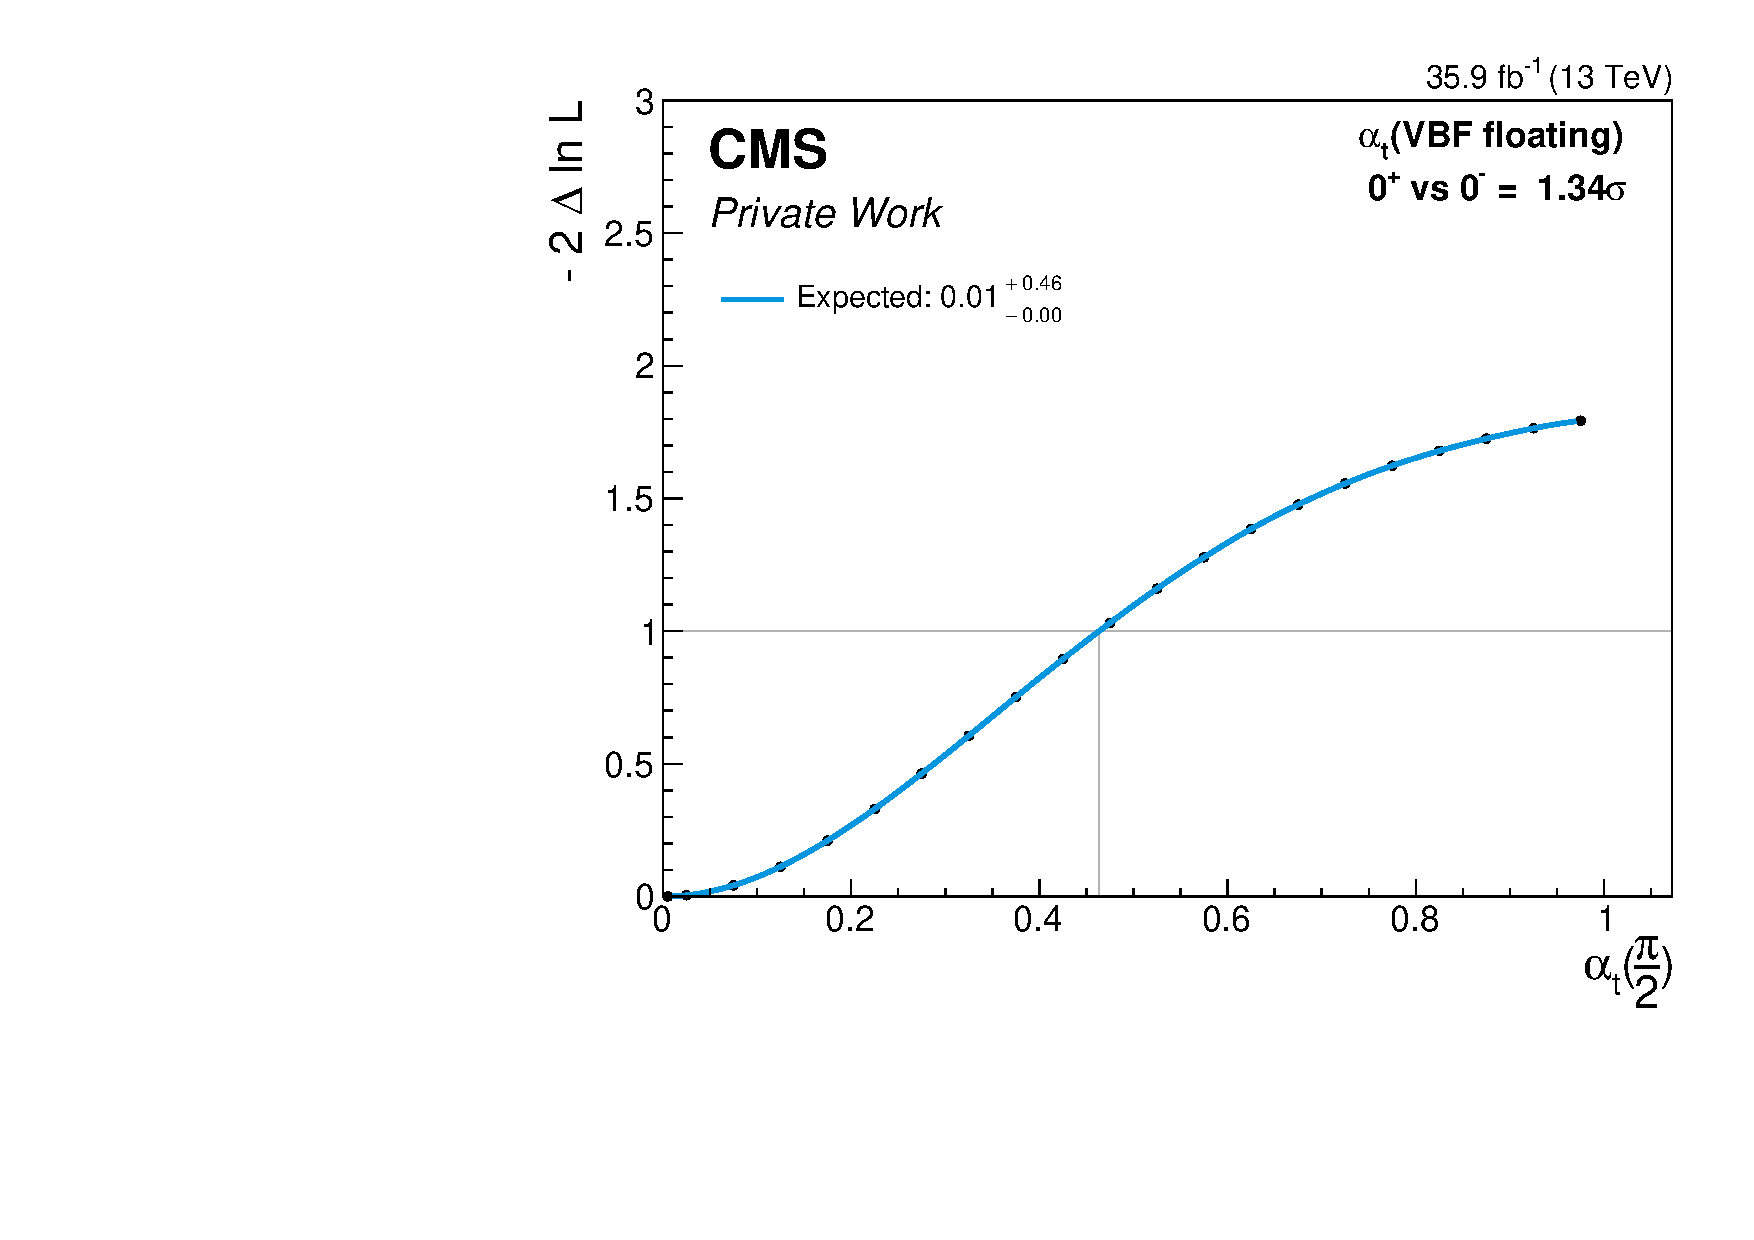
\includegraphics[width=\textwidth]{Figures/statana/Scan_JEC_mela3D/alpha_VBFfloating.pdf}
    \end{subfigure}
    \begin{subfigure}{.49\textwidth}
        \centering
        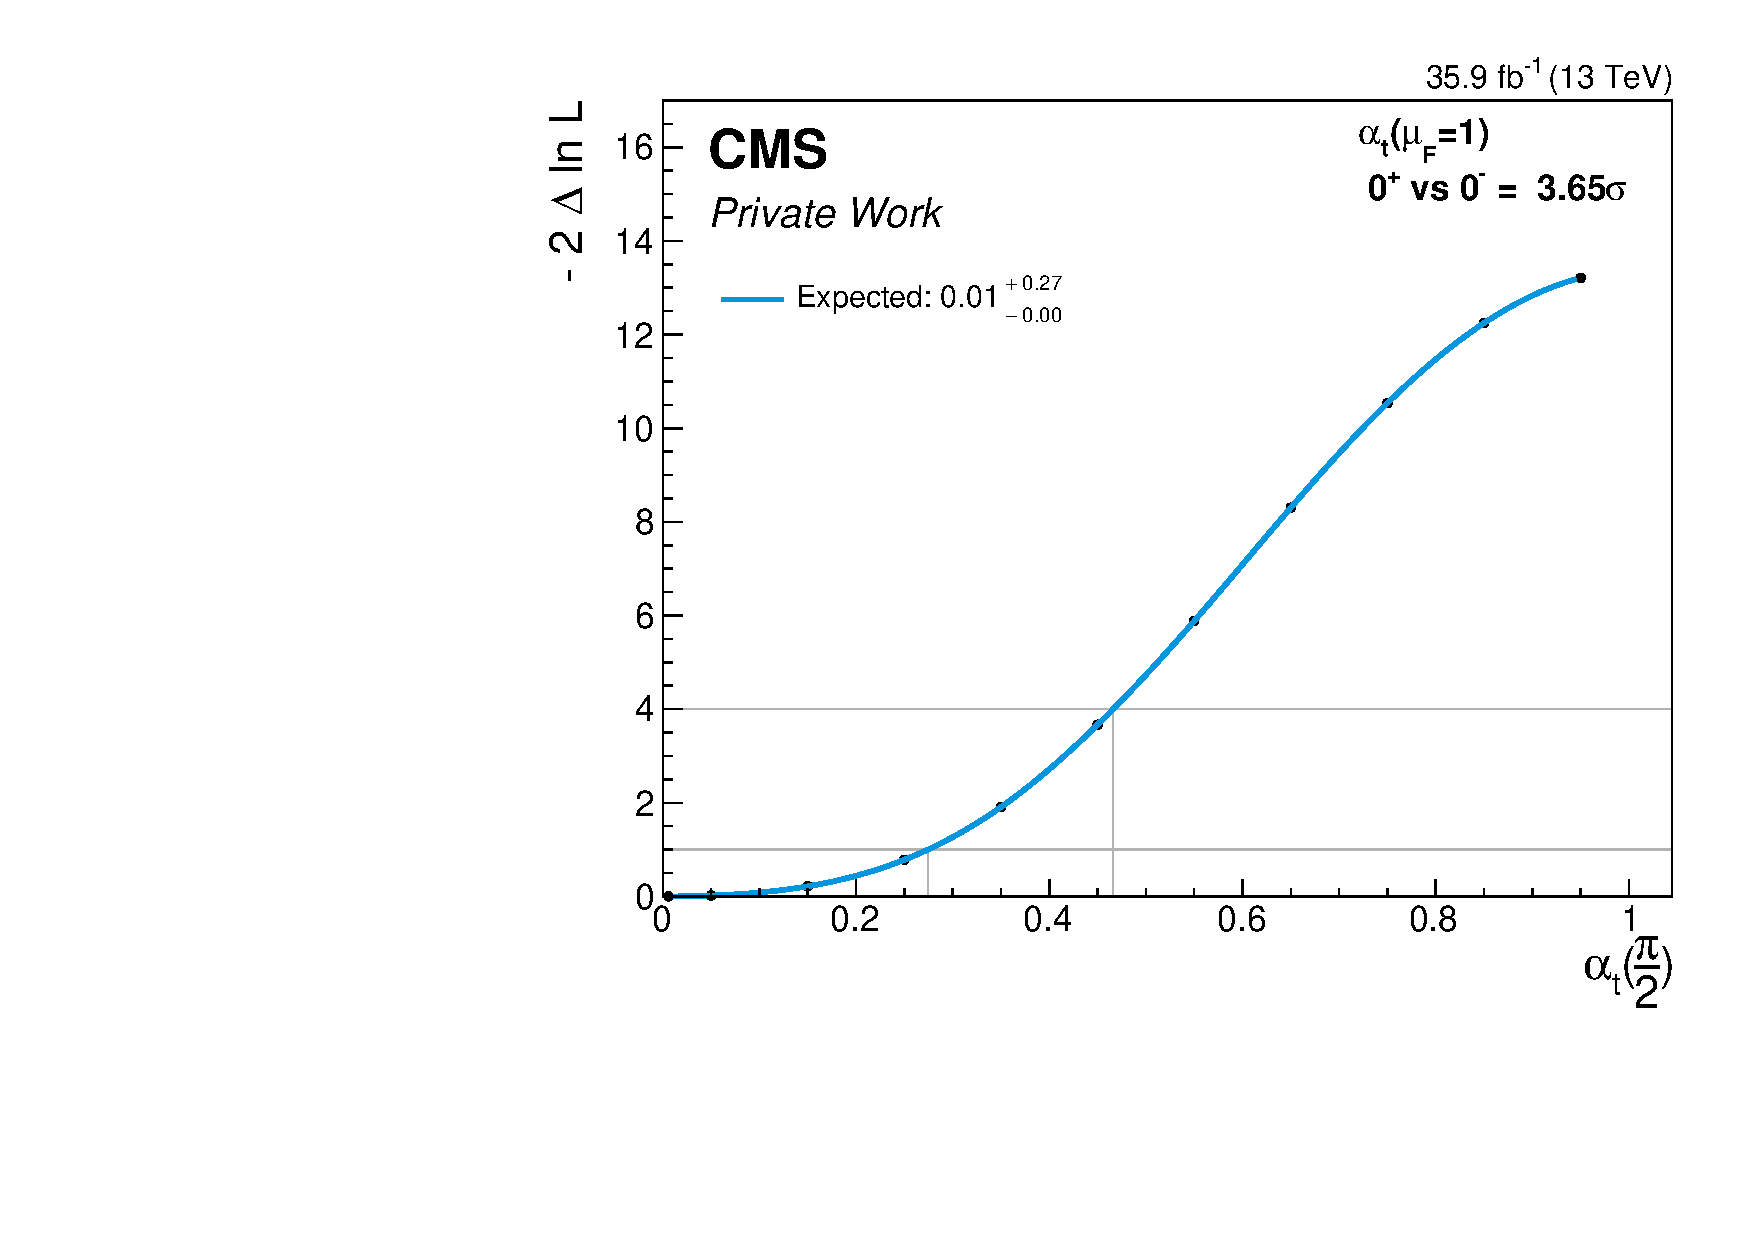
\includegraphics[width=\textwidth]{Figures/statana/Scan_JEC_mela3D/alpha_ggFconstraint.pdf}
    \end{subfigure}
    \caption[Measurement of $\alpha$ with floating VBF background and rate constraint.]{Measurement of $\alpha$ leaving the VBF CP scenario floating in the fit (left) and using the SM constraint on the ggF signal strength (right).
    No change in the accuracy of the measurement is observed compared to the nominal measurement from \figreft{statana:scan_alpha_f0} when $f$ is left floating in the fit. This justifies setting $f=0$. 
    The rate constraint leads to a better discrimination of scalar and pseudoscalar scenarios due to the expected larger coupling strength of the pseudoscalar coupling.}\label{statana:scan_alpha_ggF_VBF}
\end{figure}

\subsubsection{Uncertainty breakdown}
The analysis  is performed taking both statistical and systematic uncertainties into account. To find out the contribution of both to the final fit uncertainty and uncertainty breakdown is performed.
First, the likelihood scan with the setup used for \figreft{statana:scan_alpha_f0} is performed and the result with the total uncertainty $\sigma_\text{tot}$ stored.
The likelihood profile is repeated taking into account only statistical uncertainties by fixing the nuisance parameters to the values obtained from the stored global fit from \figreft{statana:scan_alpha_f0} this time. Thus, the result only incorporates statistical uncertainties $\sigma_\text{stat}$ as only those can float in the fit.
Using quadratic error summation the systematic uncertainty can be inferred from the the two previous measurements by
\begin{equation}
    \sigma_\text{syst} = \sqrt{\sigma_\text{tot}^2 - \sigma_\text{stat}^2}.
\end{equation} 
Both fit results and the resulting uncertainty split into a statistical and systematic component are shown in \figreft{statana:scan_alpha_breakdown}.
The total uncertainty of made of a statistical component of $\text{31.5}\degree$ and a systematic uncertainty of $\text{27}\degree$.
The measurement of $\alpha$ currently shows a larger statistical component of $0.35$ with the integrated luminosity given by the 2016 data set implying that the performance of the measurement is expected to improve when combined with the data collected in 2017 and 2018. This encourages a combination of the data sets at the end of Run 2. 


% combineTool.py -m 125 -M MultiDimFit --setParameters muF=1,muV=1,alpha=0,f=0 --freezeParameters f --setParameterRanges alpha=0,1 --points 20 --redefineSignalPOIs alpha -d /afs/desy.de/user/d/dwolfsch/cms_analysis/CMSSW_8_1_0/src/CombineHarvester/HTTSMCP2016/output/2018-09-23_FULL_mela3D_JECgroupings/cmb/125/ws.root --algo none -t -1 --there -n .alpha_bestfit --parallel=20 --saveWorkspace

\begin{figure}[h!]
    \centering
        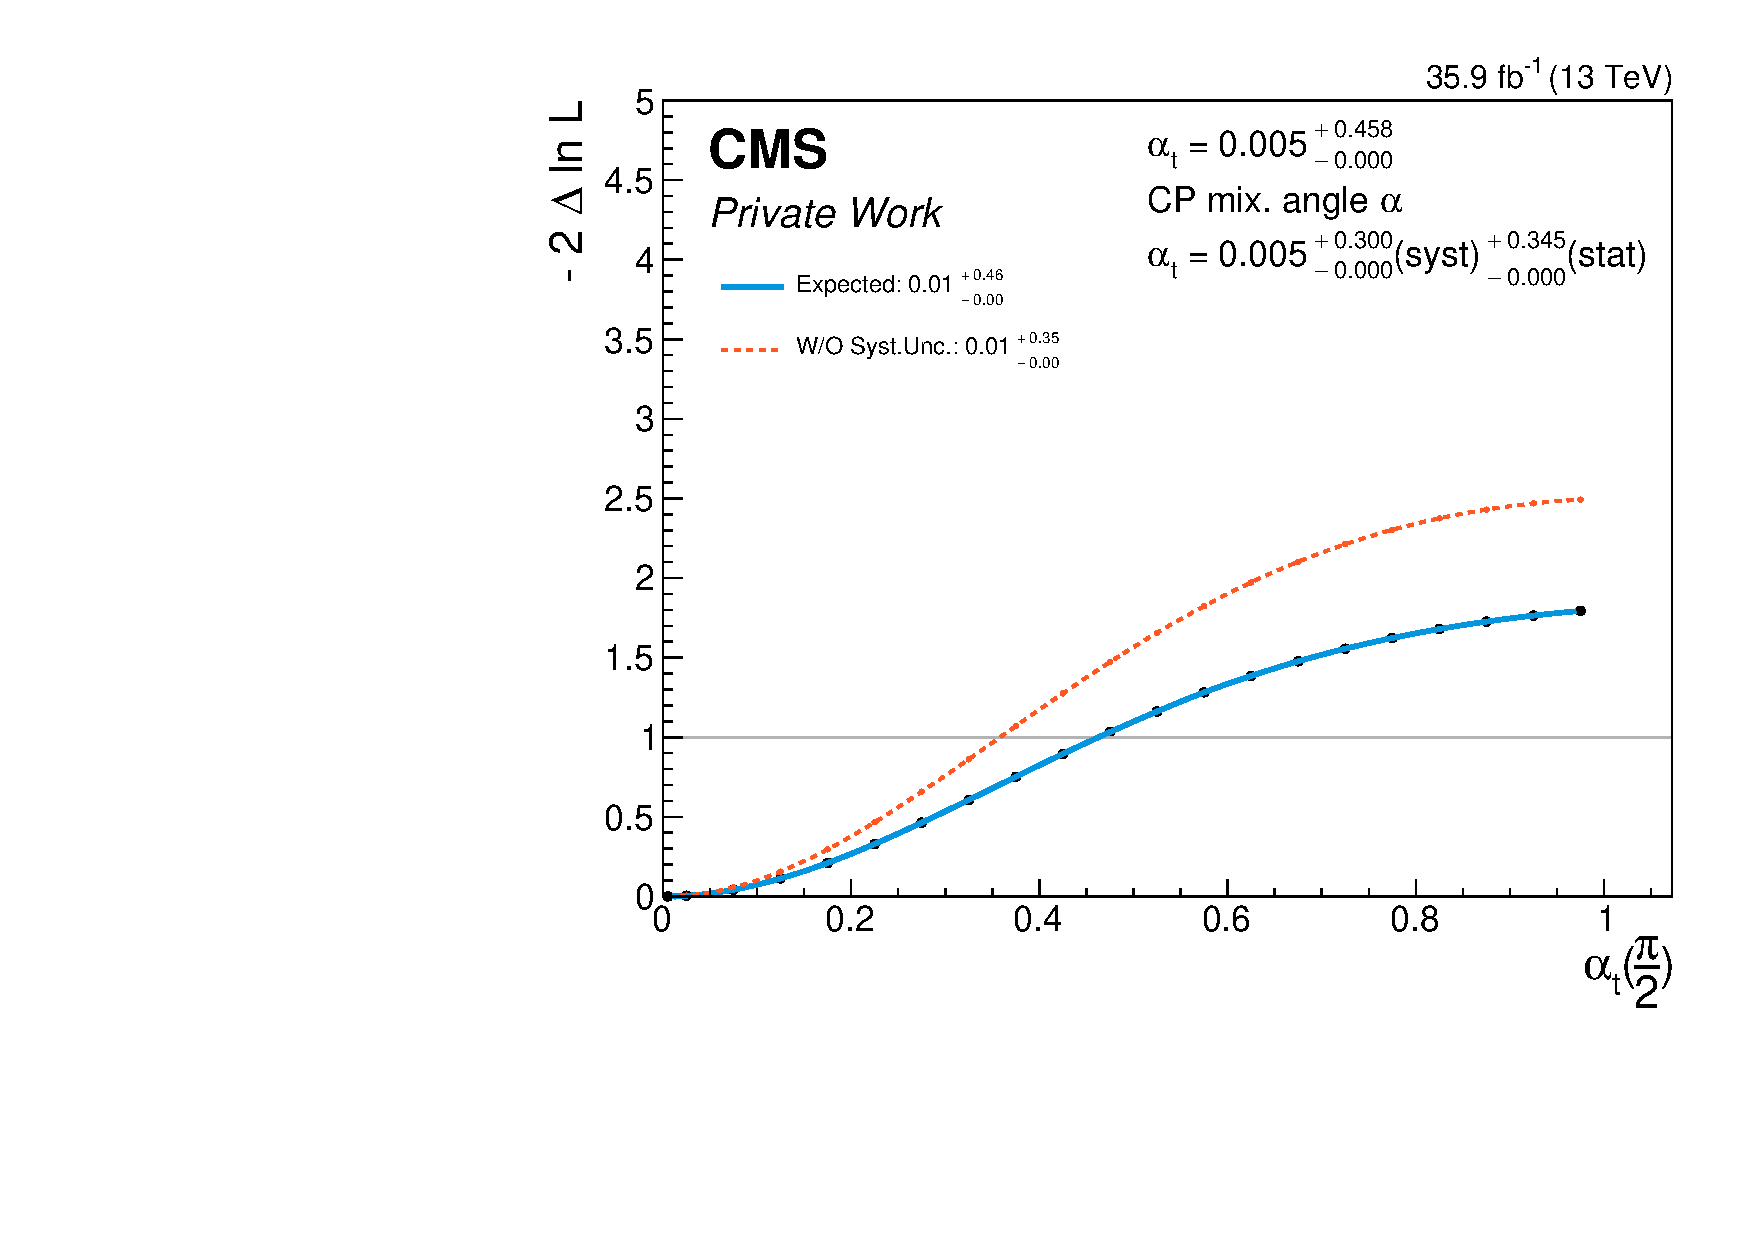
\includegraphics[width=.6\textwidth]{Figures/statana/Scan_JEC_mela3D/alpha_breakdown.pdf}
    \caption[Uncertainty breakdown of the CP mixing angle measurement.]{Final measurement of $\alpha$ stating the systematic and statistical composition of the total uncertainty on $\alpha$. With the given dataset the uncertainty of the measurement shows a larger statistical component and is thus expected to be improved with more data.}\label{statana:scan_alpha_breakdown}
\end{figure}
